\documentclass[11pt,a4paper,twoside]{report}
\usepackage{graphicx}
\usepackage{setspace}	%double spacing for text, single for captions, footnotes, etc.
%\usepackage{hypernat} 	%substitut de cite que permet fer hyperlinks
\usepackage{natbib}		% substituye a 'hypernat' que funciona en Windows.
\bibliographystyle{ksfh_nat}
\usepackage[spanish]{babel}

\usepackage[utf8]{inputenc}
\usepackage{color}
\usepackage{hhline} 		% extended styles for tables
\usepackage{multirow}
\usepackage{subfigure}
\usepackage{acronym}
\usepackage{hyperref}
\usepackage{amsmath,amsmath,amssymb} 
\usepackage{fancyhdr}
\usepackage{epsfig, amsmath}
\usepackage{algorithm}
\usepackage{algorithmic}

%% my packages
\usepackage{blindtext}
%\usepackage[toc,hyperfirst=false]{glossaries}
\usepackage{listings}
\usepackage{xcolor}
\usepackage[small]{caption}
\usepackage{subcaption}
\usepackage{url}
\usepackage{lscape}


% general settings
\hypersetup{
	linktocpage=true,
	colorlinks=true,
	linkcolor=blue,
	citecolor=blue,
	urlcolor=blue
}
\definecolor{Hgray}{gray}{0.6}

\newenvironment{definition}[1][Definition]{\begin{trivlist}
\item[\hskip \labelsep {\bfseries #1}]}{\end{trivlist}}

\setlength{\topmargin}{0cm}
\setlength{\textheight}{23cm}
\setlength{\textwidth}{17cm}
\setlength{\oddsidemargin}{0cm}
\setlength{\evensidemargin}{0cm}
\setlength{\headheight}{1cm}

% indica que las 'sub-sub-sections' sean numeradas y aparezcan en el indice
\setcounter{secnumdepth}{3}
\setcounter{tocdepth}{2}

% settings for code
\renewcommand{\algorithmicrequire}{\textbf{Entrada: }}
\renewcommand{\algorithmicensure}{\textbf{Salida: }}

%settings for listing codes
\definecolor{codegreen}{rgb}{0,0.6,0}
\definecolor{codegray}{rgb}{0.5,0.5,0.5}
\definecolor{codepurple}{rgb}{0.58,0,0.82}
\definecolor{backcolour}{rgb}{0.95,0.95,0.92}

\lstdefinestyle{mystyle}{
    backgroundcolor=\color{backcolour},   
    commentstyle=\color{codegreen},
    keywordstyle=\color{blue},
    numberstyle=\tiny\color{codegray},
    stringstyle=\color{codepurple},
    basicstyle=\ttfamily\footnotesize,
    breakatwhitespace=false,         
    breaklines=true,                 
    captionpos=b,                    
    keepspaces=true,                 
    numbers=left,                    
    numbersep=5pt,                  
    showspaces=false,                
    showstringspaces=false,
    showtabs=false,                  
    tabsize=2
}
\lstset{style=mystyle}


%%%%%%%%%%%%
% DOCUMENT %
%%%%%%%%%%%%
\begin{document}

% portada
\newpage
\thispagestyle{empty}

\baselineskip 2em

%\vspace*{1cm}

\centerline{
\includegraphics[width=0.6\textwidth]{images/UOC-logo}}
\begin{center}
\textsc{Universitat Oberta de Catalunya (UOC) \\
 Máster Universitario en Bioinformática y Bioestadística\\}

%\centerline {\pic{UOC}{4cm}}

\vspace*{1.5cm}

\textsc{\Large TRABAJO FINAL DE MÁSTER}

\vspace*{0.5cm}

\textsc{\large Subárea 12: Biología molecular y genética}


%\textbf{\Huge VirtualTechLab Model: }

\vspace*{2.0cm}

\textbf{\Large Desarrollo de herramientas bioinformáticas en Python y R para el análisis de duplicaciones génicas en bacterias y visualización de datos.}

%\textbf{\large xxx subtítulo (en caso de existir) xxx}

\vspace{2.5cm}
\baselineskip 1em

\baselineskip 2em
-----------------------------------------------------------------------------\\
Autor:      Alba Moya Garcés\\
Tutor:      José F. Sánchez Herrero\\
Profesor:   Ferran Prados\\
-----------------------------------------------------------------------------\\
\vspace*{1.5cm}
Barcelona, 5 de enero de 2021

\end{center}

\newpage
\pagestyle{empty}
\hfill

\newpage
% abstract
\pagenumbering{roman} 
\setcounter{page}{1} 
\pagestyle{plain}

%%%%%%%%%%%%%%%%
%%% CREDITOS %%%
%%%%%%%%%%%%%%%%
\chapter*{Créditos/Copyright}

Una página con la especificación de créditos/copyright para el proyecto (ya sea aplicación por un lado y documentación por el otro, o unificadamente), así como la del uso de marcas, productos o servicios de terceros (incluidos códigos fuente). Si una persona diferente al autor colaboró en el proyecto, tiene que quedar explicitada su identidad y qué hizo.

A continuación se ejemplifica el caso más habitual, aunque se puede modificar por cualquier otra alternativa:

\vspace{1cm}

\begin{figure}[ht]
    \centering
	
\includegraphics[scale=1]{images/license.png}
\end{figure}

Esta obra está sujeta a una licencia de Reconocimiento -  NoComercial - SinObraDerivada

\href{https://creativecommons.org/licenses/by-nc-nd/3.0/es/}{3.0 España de CreativeCommons}.

%%%%%%%%%%%%%
%%% FICHA %%%
%%%%%%%%%%%%%
\chapter*{FICHA DEL TRABAJO FINAL}

\begin{table}[ht]
	\centering{}
	\renewcommand{\arraystretch}{2}
	\begin{tabular}{r | l}
		\hline
		Título del trabajo: & Descriptivo del trabajo\\
		\hline
        Nombre del autor: & Nombre y dos apellidos\\
		\hline
        Nombre del colaborador/a docente: & Nombre y dos apellidos\\
		\hline
        Nombre del PRA: & Nombre y dos apellidos\\
		\hline
        Fecha de entrega (mm/aaaa): & MM/AAAA\\
		\hline
        Titulación o programa: & Plan de estudios\\
		\hline
        Área del Trabajo Final: & El nombre de la asignatura de TF\\
		\hline
        Idioma del trabajo: & Catalán, español o inglés\\
		\hline
        Palabras clave & Máximo 3 palabras clave\\
		\hline
	\end{tabular}
\end{table}

%%%%%%%%%%%%%%%%%%%
%%% DEDICATORIA %%%
%%%%%%%%%%%%%%%%%%%
\chapter*{Dedicatoria/Cita}

Breves palabras de dedicatoria y/o una cita.

%%%%%%%%%%%%%%%%%%%
%%% Agradecimientos %%%
%%%%%%%%%%%%%%%%%%%
\chapter*{Agradecimientos}

Si se considera oportuno, mencionar a las personas, empresas o instituciones que hayan contribuido en la realización de este proyecto.

%%%%%%%%%%%%%%%%
%%% RESUMEN  %%%
%%%%%%%%%%%%%%%%
\chapter*{Abstract}
\addcontentsline{toc}{chapter}{Abstract}

\onehalfspacing

Texto con la síntesis del proyecto, esto es, un texto en el cual se explica de manera concisa la definición del proyecto/problema abordado, sus objetivos/métodos de resolución, y los resultados y conclusiones (no puede ser una lista, sino un texto continuo redactado de manera estructurada). Si es necesario poner una referencia en este texto, ésta será anotada a pie de la misma página. En este apartado se puede usar un lenguaje más literario y coloquial que para el resto del documento.

El Abstract se escribirá por duplicado. Una de las versiones tiene que ser \textbf{obligatoriamente en inglés}. La otra versión tiene que estar escrita en catalán o español. En caso de no escribir el resto del documento en inglés, será necesario escribir la segunda versión del Abstract en el idioma utilizado para el resto de la memoria. La palabra Abstract se cambiará por ``\textbf{Resum}'' o ``\textbf{Resumen}'' en la versión catalana y española, respectivamente. 

Extensión recomendada: 250 palabras máximo.

Como escribir un buen Abstract (en inglés):

\href{http://www.ece.cmu.edu/~koopman/essays/abstract.html}{http://www.ece.cmu.edu/~koopman/essays/abstract.html}

\vspace{1.5cm}

\textbf{Palabras clave}: Keywords del trabajo separadas por comas. Por ejemplo para este documento podrían ser Modelo, Pauta, Plantilla, Memoria, Trabajo de Final de Grado/Máster
\newpage

\pagestyle{fancy}
\renewcommand{\chaptermark}[1]{ \markboth{#1}{}}
\renewcommand{\sectionmark}[1]{\markright{ \thesection.\ #1}}
\lhead[\fancyplain{}{\bfseries\thepage}]{\fancyplain{}{\bfseries\rightmark}}
\rhead[\fancyplain{}{\bfseries\leftmark}]{\fancyplain{}{\bfseries\thepage}}
\cfoot{}

% indice
\cleardoublepage
\phantomsection
%\addcontentsline{toc}{chapter}{Índice}
\tableofcontents
% listado de figuras
\cleardoublepage
\phantomsection
\addcontentsline{toc}{chapter}{Índice de Figuras}
\listoffigures
% listado de tablas
% \cleardoublepage
% \phantomsection
% \addcontentsline{toc}{chapter}{Índice de Cuadros}
% \listoftables





\thispagestyle{empty}



\pagestyle{fancy}
\renewcommand{\chaptermark}[1]{ \markboth{#1}{}}
\renewcommand{\sectionmark}[1]{\markright{ \thesection.\ #1}}
\lhead[\fancyplain{}{\bfseries\thepage}]{\fancyplain{}{\bfseries\rightmark}}
\rhead[\fancyplain{}{\bfseries\leftmark}]{\fancyplain{}{\bfseries\thepage}}
\cfoot{}

\onehalfspacing

% capitulos del documento
\cleardoublepage
\pagenumbering{arabic}
\setcounter{page}{1} 


\chapter{Introducción}
\label{chapter:introduccion}

\section{Contexto y justificación del trabajo}

Durante el desarrollo de este trabajo de fin de máster (TFM) se ha llevado a cabo una caracterización de las posibles duplicidades génicas presentes en los genomas de diferentes cepas bacterianas entre las especies del grupo ESKAPE no analizadas en estudios previos \textit{(Klebsiella pneumoniae, Acinetobacter baumannii, Pseudomonas aeruginosa} y  \textit{Enterobacter} spp.). Para ello se implementarán diversos módulos y paquetes específicos en los lenguajes de programación Python y R que realizarán de manera automática la búsqueda de las mismas. Con los resultados de la obtenidos, se podrán caracterizar genes específicos relacionados con virulencia o resistencia a antimicrobianos y generar gráficas para su visualización.

La duplicación genética es un proceso que se encuentra tanto en células eucariotas como procariotas y es uno de los tipos de mutación más frecuentes \cite{serres_evolution_2009,zhang_evolution_2003}. Es un mecanismo que genera una o más copias indistinguibles del mismo gen en el genoma celular y que se mantiene a lo largo de la línea evolutiva \cite{lynch_genome-wide_2008, lipinski_high_2011, sanchez-herrero_gene_2020, zhang_evolution_2003}. La ventaja evolutiva que proporciona para las bacterias mantener en sus genomas diferentes copias para el mismo gen viene determinada por que cada una de ellas podría mostrar diferentes patrones de expresión e, incluso, responder ante estímulos diferentes, lo cual dota a las cepas que portan esta variedad de copias de más oportunidades para adaptarse a variaciones fisicoquímicas del medio en el que se encuentran. El aumento de la complejidad genómica que genera esta diversidad funcional, facilita la proliferación de las células ante medios limitantes e incrementa las probabilidades de nuevas mutaciones adaptativas \cite{serres_evolution_2009,zhang_evolution_2003}.

Las bacterias del grupo ESKAPE son especialmente patógenas para los seres humanos ya que presentan en su material genético genes de resistencia a diferentes agentes antimicrobianos, lo que las hace difíciles de combatir en caso de infección \cite{lipinski_high_2011, santajit_mechanisms_2016}. La existencia de cepas patógenas multirresistentes a diferentes antibióticos ha supuesto un problema sanitario que lleva a graves consecuencias en la salud pública \cite{bernabeu_gene_2019,murray_vancomycin-resistant_2000, pendleton_clinical_2013, sanchez-herrero_gene_2020}. La limitación de los grupos científicos para crear nuevos antibióticos efectivos y la rapidez con que estas bacterias evolucionan, hace necesario aumentar los conocimientos alrededor de cómo se interrelacionan los diferentes genes bacterianos al expresarse y favorecer la supervivencia de la bacteria \cite{bernabeu_gene_2019,pendleton_clinical_2013,santajit_mechanisms_2016}.

El estudio de duplicidades génicas en \textit{E. coli}, estafilococos y enterococos ha demostrado un patrón diferenciado de las mismas entre las cepas más virulentas y las que no presentan patogenicidad. Se ha constatado la presencia de un número significativo de genes duplicados en cepas patógenas, respecto a aquellas no patógenas, que no se muestran en cepas inofensivas, lo que sugiere que estos genes podrían favorecer de forma relevante la virulencia de las mismas \cite{bernabeu_gene_2019,sanchez-herrero_gene_2020}.

La duplicación genética en bacterias se produce más frecuentemente por transferencia horizontal genética (HGT) entre diferentes individuos gracias a agentes virales, plásmidos o transposones, que por diferentes mecanismos moleculares naturales que pueden generar duplicaciones en los genomas bacterianos \cite{reams_mechanisms_2015,romero_gene_1997,sanchez-herrero_gene_2020,santajit_mechanisms_2016}. 

Identificar genes duplicados específicos en diferentes cepas patógenas, podría contribuir al estudio de los mecanismos de la virulencia de las mismas ampliando la información ya conocida sobre cómo se regula la expresión genética en las bacterias a estudio \cite{bernabeu_gene_2019,sanchez-herrero_gene_2020}. Por otro lado, si se determinara la codificación por parte de alguno de estos genes duplicados de productos antigénicos, se podrían desarrollar nuevas vacunas o medicamentos más efectivos para hacer frente a las enfermedades provocadas por este tipo de bacterias \cite{bernabeu_gene_2019, serres_evolution_2009}.

Por todo lo mencionado, en este Trabajo de TFM se complementarán los trabajos realizados por \cite{bernabeu_gene_2019} y \cite{sanchez-herrero_gene_2020} desarrollando una herramienta bioinformática capaz de llevar a cabo de manera automatizada todo el proceso de búsqueda e identificación de duplicidades dentro de un genoma dado. Se obtendría como resultado un archivo de datos con toda la información obtenida y una representación gráfica con el fin de facilitar su estudio y comprensión. Estos resultado podrán utilizarse facilmente en estudios de investigación relacionados.

Desarrollar una herramienta bioinformática, compuesta de diversos módulos específicos para cada una de las fases que comprenden el análisis genómico y la búsqueda de duplicidades, permitirá a la comunidad científica avanzar de forma más ágil en la investigación sobre el tema.



\section{Objetivos del Trabajo}

Los objetivos desarrollados a lo largo de este TFM han sido los siguientes:
\begin{itemize}
    \item Desarrollo de herramientas bioinformáticas para el análisis y caracterización de duplicidades genéticas en bacterias.
    \begin{itemize}
        \item Desarrollar funciones de python para el tratamiento y análisis de duplicaciones tanto de secuencias genómicas en bases de datos como ensambladas \textit{de novo} por parte del usuario.
        \item Implementar la generación y representación de resultados para la mejor interpretación y visualización de los datos.
    \end{itemize}
    \item Caracterización de duplicaciones génicas en una selección de cepas bacterianas.
    \begin{itemize}
        \item Selección de cepas del grupo ESKAPE para caracterizar duplicaciones génicas.
        \item Analizar las secuencias genómicas de las cepas seleccionadas y localizar e identificar genes duplicados
    \end{itemize}
\end{itemize}

\section{Enfoque y método seguido}
% Indicar cuáles son las posibles estrategias para llevar a cabo el trabajo e indicar cuál es la estrategia elegida (desarrollar un producto nuevo, adaptar un producto existente, …). Valorar porque esta es la estrategia más apropiada para conseguir los objetivos
A pesar de que ya existen trabajos previos en los cuales se muestran técnicas para el análisis de duplicidades génicas \cite{bernabeu_gene_2019, sanchez-herrero_gene_2020}, estos no presentan un desarrollo de herramientas bioinformáticas que permitan automatizar totalmente el proceso de análisis y posterior interpretación de los resultados. La estrategia que se llevará a cabo en este TFM procurará una única metodología de análisis genómico que permita a la comunidad científica realizar este proceso de una forma más directa. Cada fase del análisis, desde la lectura de los datos hasta la visualización e interpretación de resultados, se englobará en un único proceso, lo que facilitará el uso y difusión de las herramientas generadas.

En primer lugar, se han desarrollado módulos en Python \cite{Rossum_2009} para leer de manera automática la secuencia genómica proporcionada por el usuario y analizar la información indicada. Posteriormente, con la herramienta de análisis de secuencias BLAST+ \cite{madden_blast_2003}, se ha implementado otros módulos para buscar e identificar genes duplicados y generar un archivo de resultados. Los diferentes módulos creados en python se han integrado en una única herramienta que trabajará de manera automática a lo largo de todos los pasos requeridos para completar el análisis.

Finalmente, se ha creado un paquete en R \cite{R_core} para mostrar los resultados de manera interactiva con el programa BioCircos \cite{biocircos} que facilitan su interpretación. Este módulo se ha generado a partir del aportado por \cite{sanchez-herrero_gene_2020} con las modificaciones pertinentes para adaptarlo a nuestras necesidades.

Una vez desarrollada esta versión beta del programa, se ha desarrollado el segundo objetivo y analizado cepas bacterianas reales para generar resultados.


\section{Planificación del Trabajo}

% Descripción de los recursos necesarios para realizar el trabajo, las tareas a realizar y una planificación temporal de cada tarea utilizando un diagrama de Gantt o similar. Esta planificación tendría que marcar cuáles son los hitos parciales de cada una de las PEC.

Los objetivos y tareas realizados se han planteado según los diferentes hitos marcados por el plan docente. Estos hitos corresponden a cada una de las pruebas de evaluación continua (PEC) propuestas a lo largo del periodo estipulado, así como la entrega de la memoria final y la defensa pública del proyecto por medio de una presentación virtual.

La imagen \ref{fig:crono} representa la planificación del TFM. Se ha desglosado cada objetivo en las correspondientes tareas a realizar a lo largo de la línea temporal.

\begin{figure}[h]
	\centering
	\captionsetup{width=0.7\linewidth} 
	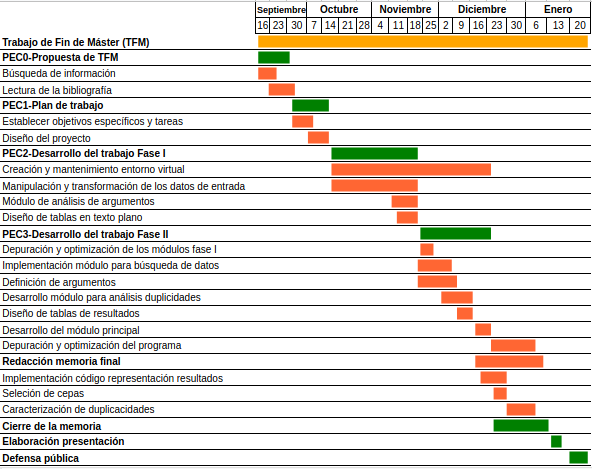
\includegraphics[width=0.7\linewidth]{figs/cronograma.png}
	\caption[Cronograma]{Cronograma detallado de la planificación del trabajo a lo largo de desarrollo del TFM. En verde se representan las entregas de documentación y en naranja las diferentes tareas realizadas.}
	\label{fig:crono}
\end{figure}
A continuación, se presenta un breve resumen de algunas de las tareas realizadas más significativas:

\begin{itemize}
    \item \textbf{Creación de un entorno virtual en Python: }para poder realizar correctamente las tareas de programación, se ha creado un espacio único para el proyecto en el que se albergue las diferentes librerías instaladas. El manejo del programa de instalación \textit{pip} ha sido fundamental para el desarrollo de este entorno. Así como el uso de aplicaciones para el control de versiones como GIT y el trabajo colaborativo en plataformas virtuales como GitHub ha favorecido la fluidez a la hora de realizar correcciones y sugerencias por parte del director de TFM y la comunicación entre ambas partes.
    
    \item \textbf{Desarrollo de módulos básicos: }Se han creado las diferentes funciones necesarias para implementar el módulo para la búsqueda de datos. Estos módulos básicos se han concebido como pequeños fragmentos de código funcionales capaces de realizar las diferentes acciones de manipulación y transformación de los datos proporcionados. De esta forma, se obtendrán objetos que puedan ser utilizados en el módulo principal. Se han utilizado herramientas en BioPython profundizando en la documentación proporcionada para cada función y adaptándolas a nuestras necesidades para la creación de los nuevos programas.
    
    \item \textbf{Transformación de la información a texto plano: }mediante los programas Pandas y Numpy, se han manipulado los archivos de anotación genómicos (e.g. genbank, GTF, GFF) para crear objetos de python con la estructura adecuada para generar tablas y poder volcarlas como texto plano y visualizarlas, por ejemplo, en un procesador de hojas de cálculo. Estas tablas se han utilizado posteriormente para analizar las duplicidades génicas de los genomas estudiados.
    
    \item \textbf{Depuración de los módulos creados: }durante la primera fase del proyecto, se generaron una serie de módulos que debían ser depurados para su correcto funcionamiento. El seguimiento de errores de programación y su resolución han llevado un tiempo necesario para que el funcionamiento de los siguientes módulos asociados fuera correcto. Se ha implementado el programa de forma que sea muy flexible en cuanto al tipo de información proporcionada por el usuario.
    
    \item \textbf{Definición de argumentos: }para desarrollar una herramienta versátil y de fácil manejo por parte del usuario, se debe ofrecer un amplio rango de posibilidades que faciliten su uso sea cuál sea el tipo de archivo que se utilice para la búsqueda de duplicidades. Así, se han previsto distintos escenarios para definir los argumentos posibles y generar los resultados en una única línea de comandos en la consola LINUX.
    
    \item \textbf{Diseño de tablas de resultados: }mediante los programas Pandas y Numpy se han definido los archivos de texto plano para formatear las tablas con los resultados obtenidos.
    
    \item \textbf{Desarrollo del módulo principal: }Para posibilitar la búsqueda de duplicidades en solo una línea de comando en la terminal, todos los módulos programados previamente deben relacionarse entre sí para poder funcionar como un conjunto. Este módulo principal recogerá los argumentos proporcionados por el usuario y, en base a ello, utilizará unas funciones u otras para generar el archivo de resultados.
    
    \item \textbf{Implementación del código para la representación de resultados: }Implementación del módulo en R que permitirá representar los resultados. Con el paquete BioCircos se ha diseñado un script adaptado a las peculiaridades de los datos generados por el programa en python para generar gráficos representativos del genoma estudiado y los diferentes grupos de duplicados relacionados entre sí.
\end{itemize}












\section{Breve sumario de productos obtenidos}
% No hay que entrar en detalle: la descripción detallada se hará en el resto de capítulos. 

Durante el periodo de realización del TFM se han entregado los siguientes documentos:

\begin{itemize}
    \item Propuesta de TFM.
    \item Pruebas de evaluación contínua:
    \begin{itemize}
        \item Definición de los contenidos del trabajo.
        \item Plan de trabajo.
        \item Informes de seguimiento
    \end{itemize}
\end{itemize}

A estos documentos, se deben añadir la presente memoria y la presentación y defensa del TFM. Finalmente, se realizará un informe de autoevaluación que también será entregado con el resto de documentación.

Además de estos documentos, se han obtenido los siguientes productos:

\begin{itemize}
    \item Secuencias de comandos (scripts) de los módulos en python.
    \item Script del programa en R.
    \item Tablas de anotación y gráficos de las duplicidades génicas de las cepas seleccionadas.
    \item Repositorio público en github con todos los scripts desarrollados, documentación y resultados generados. ******incluir link cuando esté todo listo****
\end{itemize}

\section{Breve descripción de los otros capítulos de la memoria}
El capítulo \ref{chapter: desarrollo} se ha dedicado a explicar detalladamente cada módulo desarrollado y su funcionamiento. Cada una de las secciones del capítulo corresponde a las diferentes fases del proceso, desde la entrada de datos hasta la generación de resultados y su representación gráfica.

El capítulo \ref{chapter: analisis} describe el uso de las herramientas creadas para el análisis de duplicidades en cepas bacterianas seleccionadas. 

El apédice \ref{apA} contiene información sobre los requerimientos necesarios para utilizar los módulos implementados. Se resume brevemente los programas complementarios que se deben instalar y los enlaces al repositorio en github para la descarga de los scripts completos.

Por último, el apéndice \ref{apB} incluye los resultados obtenidos en el análisis de las cepas seleccionadas.
\chapter{Desarrollo de herramientas bioinformáticas para el análisis de duplicidades genéticas}
\label{chapter: desarrollo}

% En estos capítulos, hay que describir los aspectos más relevante del diseño y desarrollo del proyecto, así como de los productos obtenidos. La estructuración de los capítulos puede variar según el tipo de Trabajo.  

% En cada apartado es muy importante describir las alternativas posibles, los criterios utilizados para tomar decisiones y la decisión tomada.

% En caso de que corresponda, se incluirá un apartado de “Valoración económica del trabajo”. Este apartado indicará los gastos asociados al desarrollo y mantenimiento del trabajo, así como los beneficios económicos obtenidos. Hacer un análisis final sobre la viabilidad del producto.


%% añadir una primera fase que resuma todo

%% Ejemplo:
Para poder realizar una búsqueda de genes duplicados contenidos en un genoma se requiere obtener la información tanto de la anotación como de la secuencia proteica de cada gen codificante. Para ello es necesario un preprocesado de la información contenida en los diferentes ficheros de anotación y una posterior búsqueda de secuencias duplicadas. Posteriormente se representa toda esta información generada en un gráfico que muestre las relaciones entre las duplicaciones encontradas y su situación dentro del genoma.

A continuación se detalla cada fase del proceso y el desarrollo de las herramientas creadas para realizar cada tarea. Todo el código generado y la documentación necesaria para replicar el trabajo hecho se puede encontrar en el siguiente repositorio de github:

************************ link github

%% hacer referencia al github y poner link



En la figura \ref{fig:workflow} se muestran los pasos del proceso de análisis desde la entrada de información hasta la generación resultados y gráficos.

\begin{figure}[h]
	\centering
	\captionsetup{width=\linewidth} 
	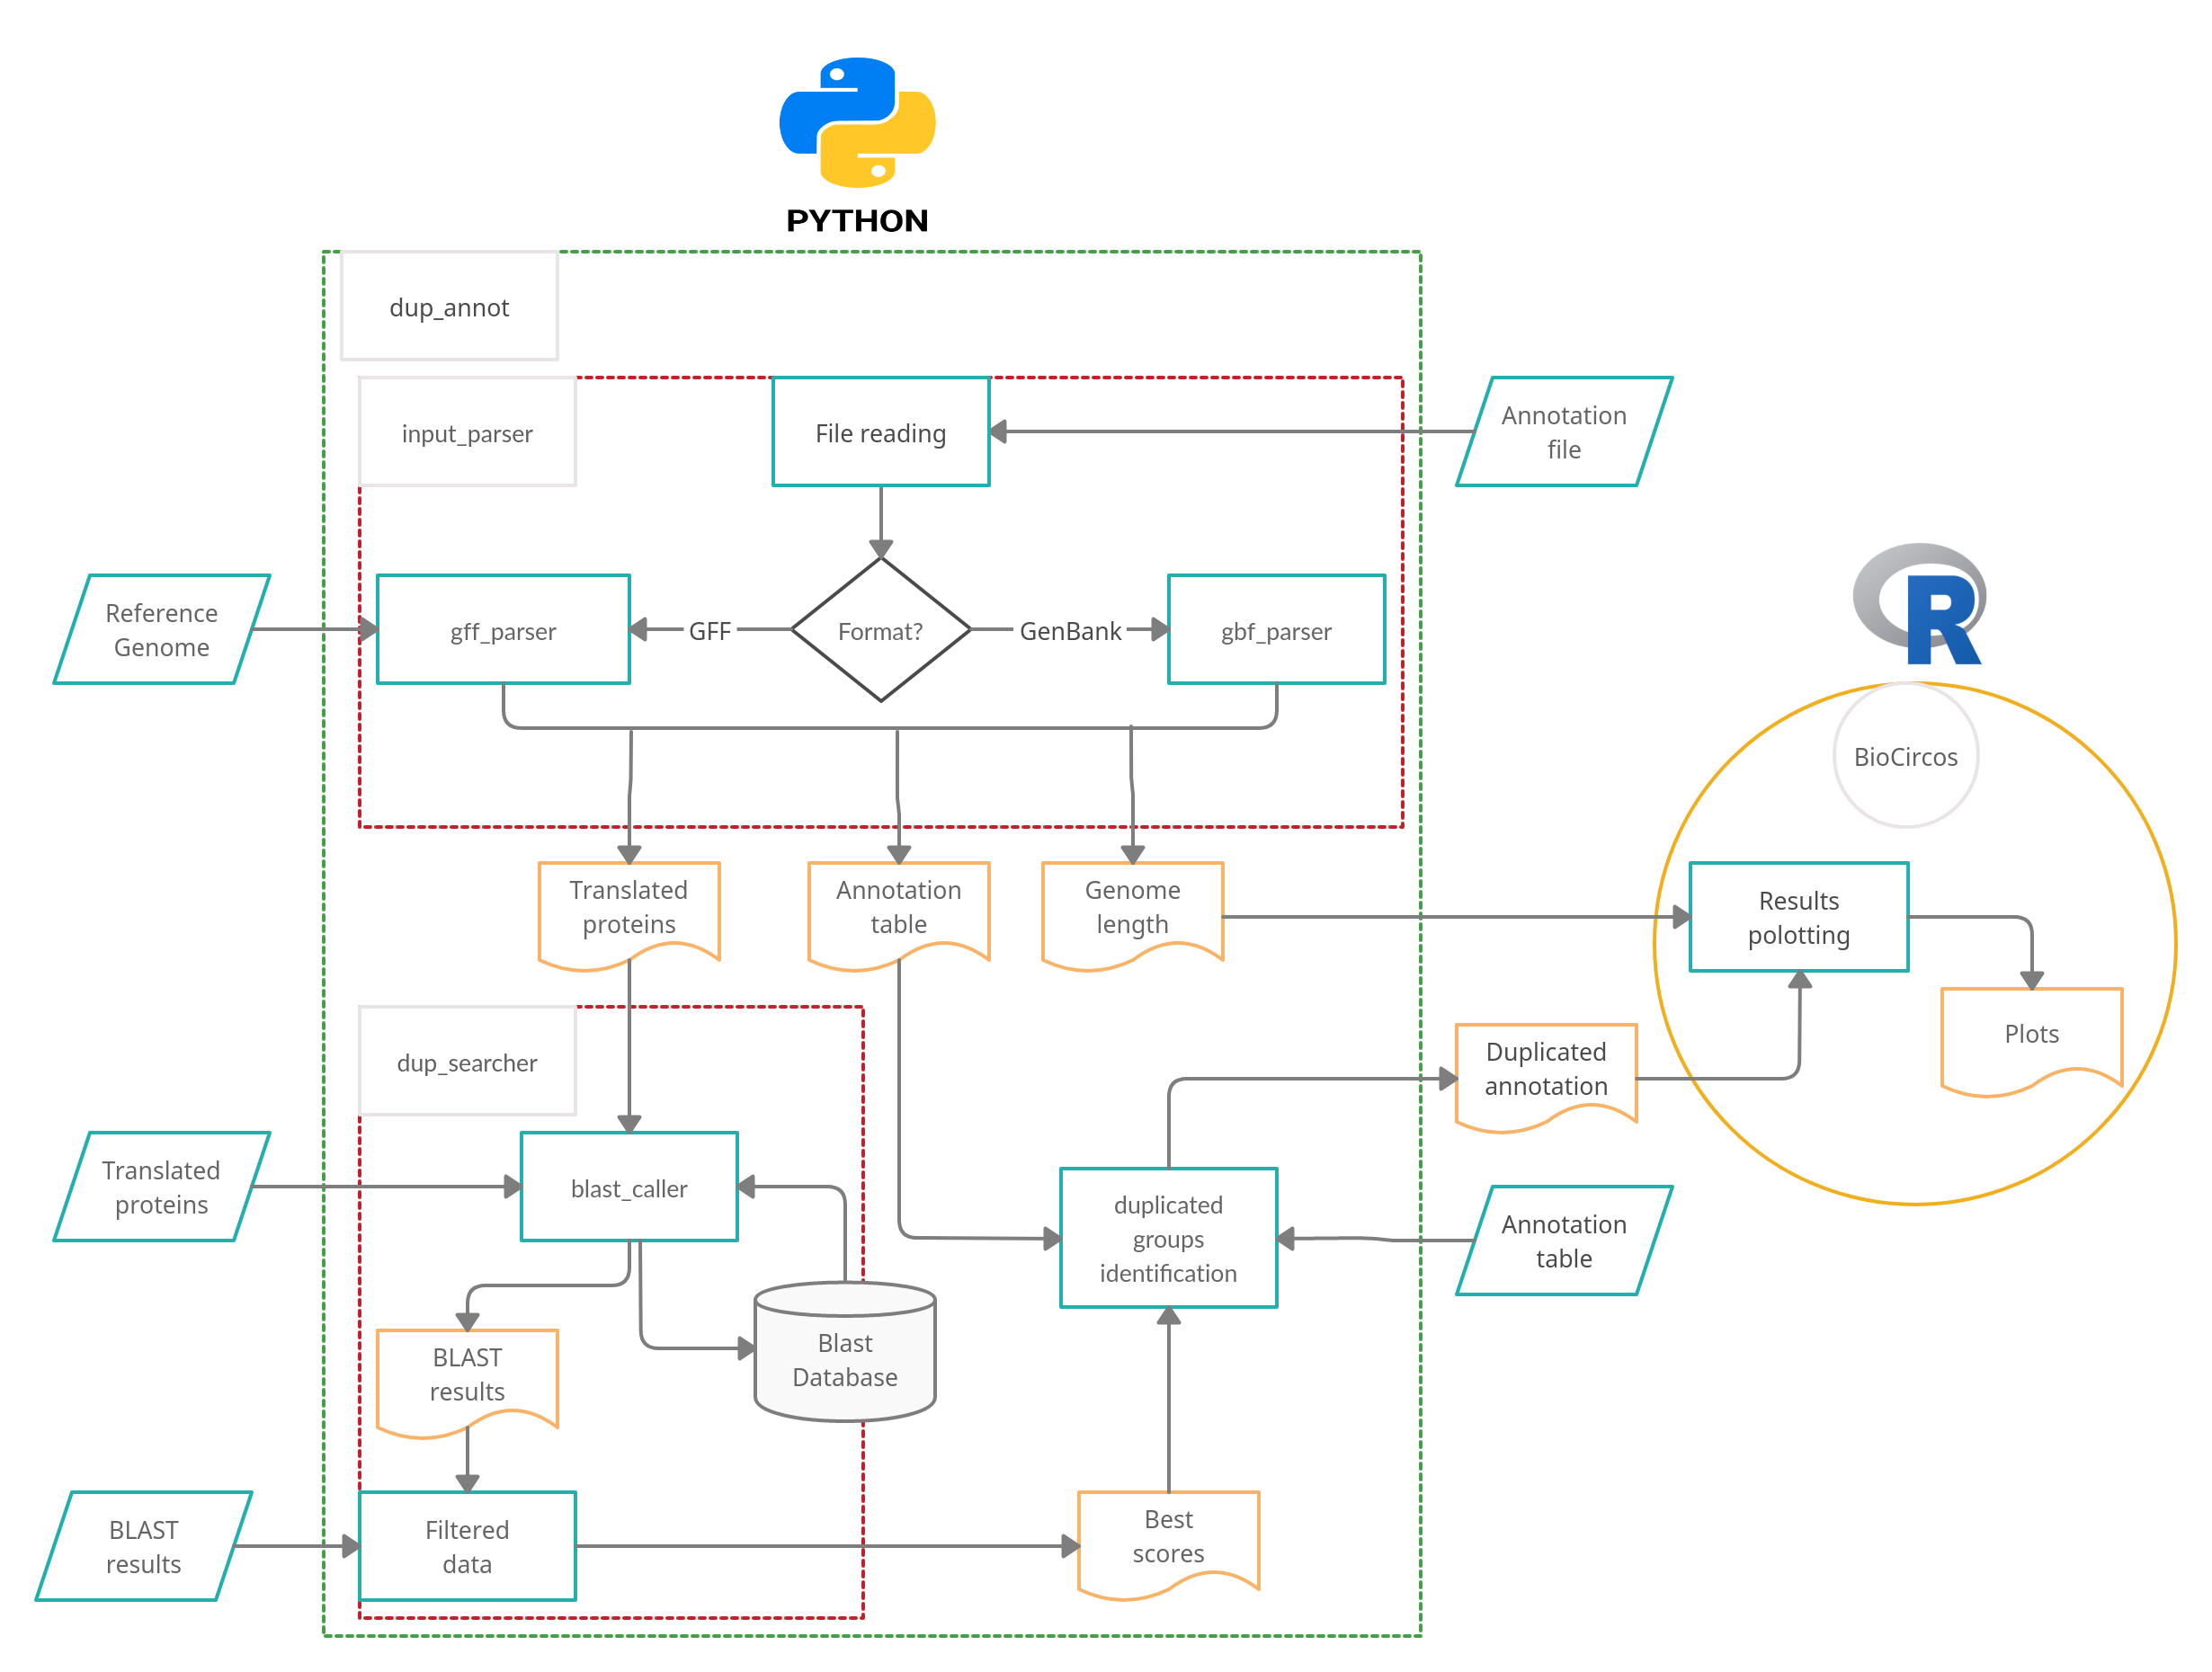
\includegraphics[width=\linewidth]{figs/workflow.png}
	\caption[Diagrama de flujo de datos de los programas desarrollados]{Diagrama de flujo de datos de los programas desarrollados donde puede seguirse el recorrido de los datos desde que entran en el programa hasta que se generan los resultados. Los paralelogramos corresponden a entrada de información desde el exterior (usuario); los rectángulos identifican cada función en python que desarrolla el proceso; las líneas de puntos engloban los módulos que contienen las correspondientes funciones en python; los círculos engloban los procesos desarrollados en R.}
	\label{fig:workflow}
\end{figure}

\section{Módulos en $python$}

\subsection{Requerimientos}

% añadido
El objetivo de este proyecto es comenzar el desarrollo de un paquete de python que permita la generación de análisis de duplicaciones a partir de ficheros de anotación. Para el desarrollo y testado de este paquete se ha utilizado la versión 3.8.5 de python y creado un entorno virtual específico para el TFM con el siguiente comando:

%% dejar espacio

%% a mi personalmente me gusta mas en gris que en negro 
% pues que se haga el gris

\vspace{5mm}

\colorbox{gray}{\textcolor{white}{\$ mkdir environments}}

\colorbox{gray}{\textcolor{white}{\$ cd environments}}

\colorbox{gray}{\textcolor{white}{\$ python3 -m venv TFM}}    

\vspace{5mm} %% espacio

Seguidamente, se instala el paquete de instalación $pip$ que nos permitirá descargar módulos específicos necesarios para el funcionamiento de nuestro programa.

\vspace{3mm}
\colorbox{gray}{\textcolor{white}{\$ sudo apt install -y python3-pip}}
\vspace{3mm}

En el apéndice \ref{apA} se facilita la lista de módulos instalados a lo largo del desarrollo del programa y una breve descripción de los módulos instalados con $pip$.

%% añadido
Para la generación de búsquedas de similitud de secuencias, necesitamos hacer uso de BLAST+, en concreto de la herramienta Blastp, la cual compara secuencias de proteína a estudio con una base de datos de proteínas de referencia \cite{bethesda_md_national_library_of_medicine_us_blast_nodate,altschul_basic_1990}. En el apéndice \ref{apA} se muestra su instalación y funcionamiento desde el terminal \cite{bethesda_md_national_center_for_biotechnology_information_us_blast_2008}.

\subsection{Entrada de datos e información}

La información proporcionada por el usuario puede ser de diferentes tipos y presentarse en diferentes formatos:

\begin{itemize}
\item \textbf{Anotación y ensamblaje de un genoma:} Pueden provenir de una base de datos RefSeq o GenBank como la de \textit{National Center for Biotechnology Information} (NCBI) \cite{national_center_for_biotechnology_information_national_1988} o haber sido ensambladas \textit{de novo}. Nuestro programa admitirá dos tipos de formatos que incluyan la anotación del genoma:  \href{https://www.ncbi.nlm.nih.gov/Sitemap/samplerecord.html}{GenBank} y \href{https://www.ncbi.nlm.nih.gov/Sitemap/samplerecord.html}{GFF3}, este último deberá ir acompañado de un archivo \href{https://blast.ncbi.nlm.nih.gov/Blast.cgi?CMD=Web&PAGE_TYPE=BlastDocs&DOC_TYPE=BlastHelp}{fasta} que contenga la secuencia genómica de referencia correspondiente mientras que los archivos en formato GenBank, ya tienen incluida esta información al final del documento.

\item \textbf{Proteínas de interés:} Archivo en formato fasta con las proteínas traducidas. Pueden provenir de trabajos previos. Deben ir acompañadas de un archivo $csv$ con la anotación del genoma.
\item \textbf{Tabla de anotación:} Archivo en formato $csv$ en el que aparezca la anotación del genoma a estudio. Debe ir acompañado de un archivo fasta con las secuencias proteicas.
\end{itemize}

Dependiendo del tipo de información, el tratamiento de la misma será diferente.

\subsection{Tratamiento de datos de anotación: input\_parser.py}

Como se puede apreciar en la figura \ref{fig:usage_input_parser}, el módulo input\_parser.py se define con una serie de argumentos necesarios para activar el proceso. En caso de no proporcionar aquellos obligatorios (archivo de anotación y carpeta de salida donde se guarden los archivos generados) se generará un error que no permitirá continuar (Figura \ref{fig:error_input_parser}). 


\begin{figure}[h]
\centering
    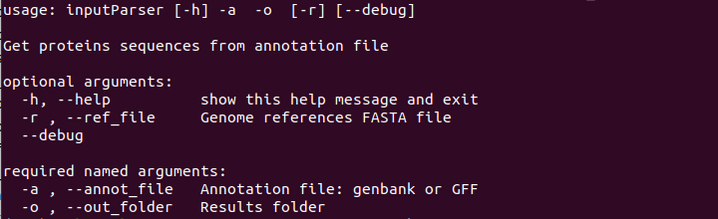
\includegraphics[width=0.7\textwidth]{figs/usage_input_parser.png}
    \caption[Información del uso de input\parser en la terminal]{Información del uso de argumentos de input\_parser.}
    \label{fig:usage_input_parser}
\end{figure}


Este módulo se encarga. en primer lugar, de tomar los ficheros de entrada y determinar su formato. En función de la extensión del archivo, llamará a la función que analiza archivos GFF o GenBank. Si la extensión no se incluye dentro de un listado determinado, se generará un error y el programa no continuará el proceso. 

\begin{figure}[h]
	\centering
	\captionsetup{width=0.7\linewidth} 
	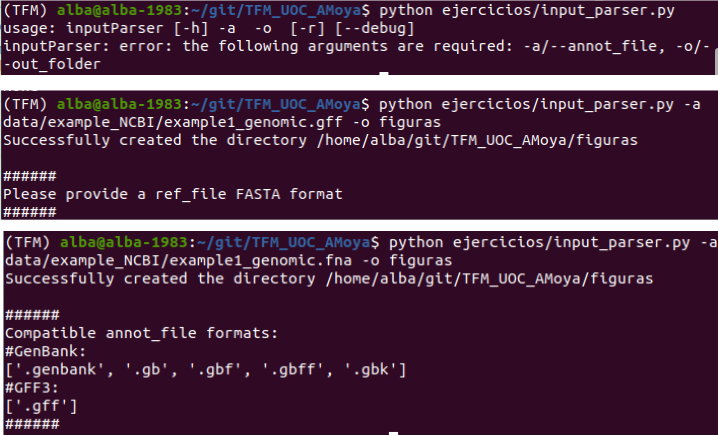
\includegraphics[width=0.7\linewidth]{figs/error_input_parser.png}
	\caption[Errores en input\_parser.py]{Diferentes errores que pueden ocurrir: Falta de carpeta de salida (arriba) o de archivo de referencia genómica (centro) y formato incorrecto (abajo).}
	\label{fig:error_input_parser}
\end{figure}

%% Añadido
Puesto que la información contenida en cada tipo de fichero de anotación esta estructurada de forma diferente el manejo de esta debe ser acorde a sus características. Si tenemos un archivo GenBank, se llamará a \textbf{gbf\_parser.py} para que lleve a cabo la conversión de los datos a las secuencias de proteínas traducidas. Además, generará un fichero de texto plano con la información contenida en el archivo de anotación en forma de tabla. Si, en cambio, tenemos un archivo GFF, se invocará a \textbf{gff\_parser.py}, el cual necesitará que también se facilite el archivo de referencia genómica para poder producir el archivo de proteínas. Si este segundo archivo no se proporciona, el programa detectará un error y no continuará el proceso (Figura \ref{fig:error_input_parser}).


Al terminar el proceso, obtendremos una carpeta de salida con tres documentos:

\begin{itemize}
\item df.csv: tabla de anotación del genoma que se utilizará (Figura \ref{fig:annot_table}). Está formada por 13 columnas de anotación que describen a cada una de las id únicas (protID) generadas por el programa para cada entrada. 

\begin{figure}[h]
	\centering
	\captionsetup{width=\linewidth} 
	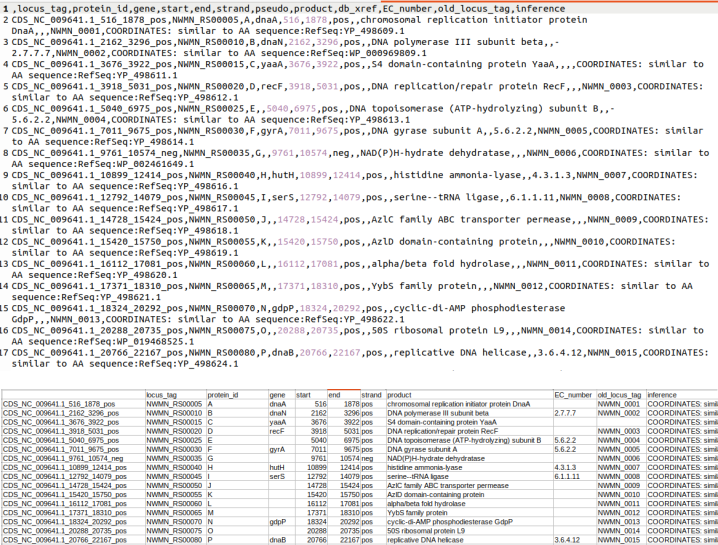
\includegraphics[width=\linewidth]{figs/annot_table.png}
	\caption[Tabla de anotación del genoma]{Tabla de anotación generada tras el tratamiento de los datos con input\_parser.py.}
	\label{fig:annot_table}
\end{figure}


\item proteins.fa: archivo en formato fasta con las secuencias proteicas provenientes de la traducción de las diferentes regiones de codificación del genoma (CDS)
\item length.csv: tabla en la que se incluye los diferentes identificadores de secuencia contenidos en los archivos de anotación proporcionados y su tamaño en pares de bases (pb).
\end{itemize}

\subsection{Comparación de secuencias con BLAST+: blast\_caller.py}
%% pequeña introductocción de que hace
BLAST+ (\textit{Basic Local Alignment Search Tool}) es una herramienta informática de alineamiento de secuencias. Puede realizar búsquedas en las bases de datos de secuencias en cuestión de segundos para encontrar similiritudes con las secuencias problema alineándolas por pares. Hay cinco variantes del algoritmo dependiendo del tipo de secuencias que se comparen entre sí: blastp para comparaciones entre proteínas; blastn compara secuecias de nucleótidos; blastx y y tblastn entre las posibles traducciones de secuencias de nucleótidos y bases de datos de proteínas y tblastx compara las seis traduciones posibles en sus marcos de lectura de la secuencia problema contra la seis de las secuencias de la base de datos de nucleótidos \cite{madden_blast_2003, altschul_basic_1990}.

Como se ha comentado al inicio del capítulo, utilizaremos la herramienta Blastp a nivel local. Es decir, invocaremos al algoritmo con los parámetros adecuados para que utilice como bases de datos las mismas secuencias de proteínas con las que después tratará de encontrar los mejores alineamientos. Cada uno de estos alineamientos obtendrá una puntuación de calidad que indicarán el grado de similitud de las dos secuencias comparadas \cite{madden_blast_2003, altschul_basic_1990}.
%% explicar que se hace una busqueda de las propias proteinas consigo mismas para buscar duplicados internamente

El módulo blast\_caller.py se divide en dos fases:

\begin{itemize}
\item \textbf {Generación de la base de datos} local a partir del archivo de proteínas generado anteriormente.
\item \textbf {Generación resultados BLAST} comparando las secuencias de la base de datos con el mismo archivo de proteínas (las secuencias se comparan entre sí mismas dos a dos).
\end{itemize}

Este módulo se define con los argumentos requeridos y opcionales mostrados en la figura \ref{fig:usage_blast_caller}. Es necesario que el usuario aporte un archivo fasta de proteínas para que el programa funcione. Además, se debe añadir la ruta donde se encuentran los archivos ejecutables de BLAST para que puedan ser utilizados.

\begin{figure}[h]
\centering
    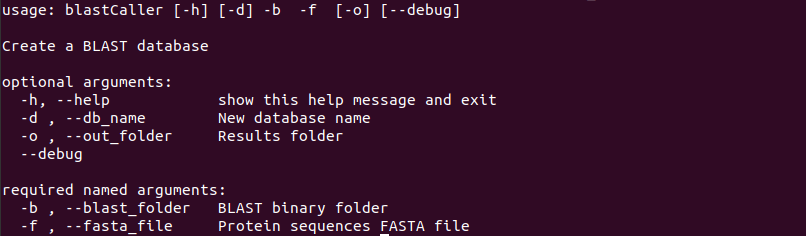
\includegraphics[width=0.7\textwidth]{figs/usage_blast_caller.png}
    \caption[Información de blast\_caller en la terminal]{Información del uso de argumentos de blast\_caller}
    \label{fig:usage_blast_caller}
\end{figure}

%% modificado
El programa permite generar el comando necesario para ejecutar BLAST+ haciendo una llamada al sistema utilizando la funcion \textit{system} de python (Figura \ref{fig:blast_caller}).

\begin{figure}[h]
	\centering
	\captionsetup{width=0.7\linewidth} 
	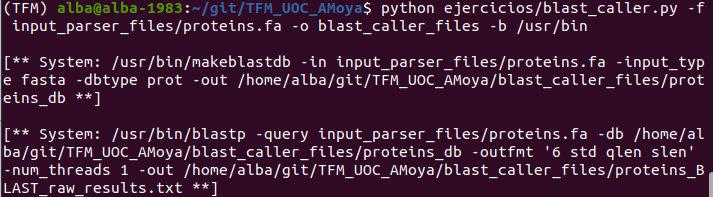
\includegraphics[width=0.7\linewidth]{figs/blast_caller.png}
	\caption[Linea de comandos blast]{Linea de comandos en la terminal para ejecutar makeblastdb y blastp}
	\label{fig:blast_caller}
\end{figure}

Al finalizar el proceso, por un lado, se obtienen tres archivos proteins\_db que forman la base de datos de proteínas, donde las extensiones \textit{phr}, \textit{pin} y \textit{psq} corresponden a las cabeceras, índices y secuencias, respectivamente. 

Por otro lado, obtenemos un fichero de con los resultados BLAST en bruto de las secuencias similares obtenidas (hits). Este último documento se presenta como una tabla con las siguientes columnas \cite{scholz_blastn_nodate, scholz_e-value_nodate}:

- id de la secuencia problema

- id de la secuencia de referencia

- porcentaje de coincidencias idénticas

- longitud del alineamiento

- número de no concordancias 

- número de huecos

- comienzo del alineamiento en la secuencia problema

- final del alineamiento en la secuencia problema

- comienzo del alineamiento en la secuencia de referencia

- comienzo del alineamiento en la secuencia de referencia

-  e-valor: número de hits de igual calidad que se espera encontrar debido al azar. Los resultados aparecen ordenados por defecto según su e-valor, los mejores hits (valores más bajos) aparecen primero. Por defecto, se establece en un valor de 10, por encima del cual los alineamientos no se incluyen en el documento.

- bit-score: tamaño de una base de datos requerido para encontrar el mismo número de concordancia por azar. Las secuencias presentan mayor similitud cuanto mayor sea su bit-score.

- longitud de la secuencia problema

- longitud de la secuencia de referencia

\subsection{Búsqueda de duplicados: dup\_searcher.py}

Este módulo ofrece dos posibilidades de datos de entrada. El usuario puede proporcionar el archivo fasta de proteínas, que hará que el módulo conecte con blast\_caller para generar el documento de resultados. O bien, puede proporcionar directamente un documento de resultados BLAST creado previamente.

Los argumentos definidos para dup\_searcher (figura \ref{fig:usage_dup_sarcher}) nos permite cambiar las variables de filtrado de los datos para generar unos resultados más o menos afinados.
Así, podemos cambiar los valores mínimos de bit-score, e-valor o los porcentajes de alineamiento o similitud, por debajo de los cuales serán eliminados de la lista de resultados. Paralelamente, se filtran las parejas espejo (cuando A=B y B=A) y las que correspondan a una secuencia alineada consigo misma (A=A). Por defecto, se ha diseñado el programa para trabajar con un e-valor $=10^{-05}$ (un e-valor bajo nos permitirá tener pocos resultados pero de buena calidad), bit-score = 50 y unos porcentajes de alineamiento y similitud del 85\%.

\begin{figure}[h]
\centering
    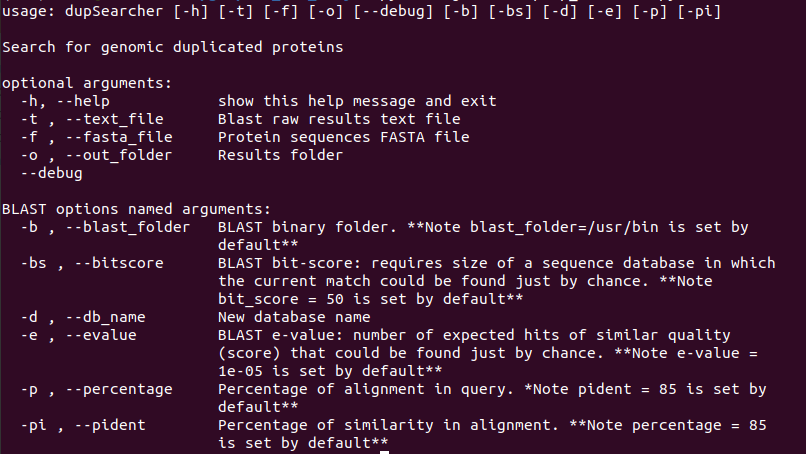
\includegraphics[width=0.7\textwidth]{figs/usage_dup_searcher.png}
    \caption[Información de dup\_searcher en la terminal]{Información del uso de argumentos de dup\_searcher}
    \label{fig:usage_dup_sarcher}
\end{figure}


El resultado final es una tabla ordenada según el porcentaje de alineamiento en primer lugar, seguido por un orden ascendente de  e-valor (los mejores resultados, e-valor menor, primero) y bitscore en sentido descendente. Añadimos los encabezados de las columnas y obtenemos un documento similar a la figura \ref{fig:dup_annot}

\begin{figure}[h]
	\centering
	\captionsetup{width=\linewidth} 
	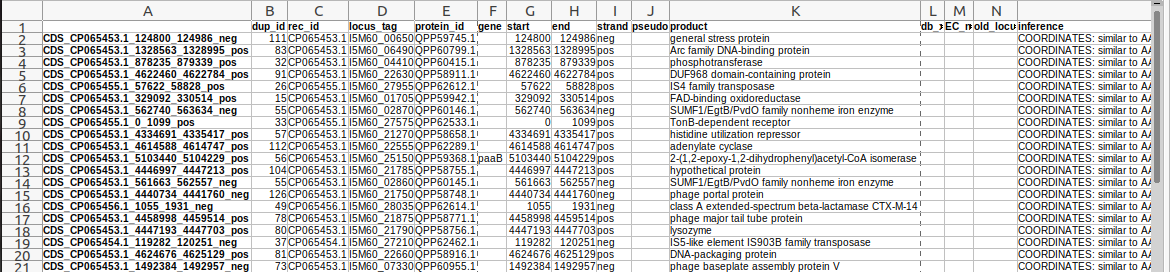
\includegraphics[width=\linewidth]{figs/dup_annot.png}
	\caption[Tabla de anotación del genoma]{Tabla de anotación generada tras el tratamiento de los datos con input\_parser.py}
	\label{fig:dup_annot}
\end{figure}


\subsection{Anotación de las proteínas duplicadas: dup\_annot.py}
Este módulo engloba a todos los anteriores. Los argumentos definidos (figura \ref{fig:usage_dup_annot}) lo dotan de la flexibilidad necesaria para generar los resultados independientemente del tipo de información proporcionada, iniciando el proceso a partir del punto correspondiente según la misma.

\begin{figure}[h]
\centering
    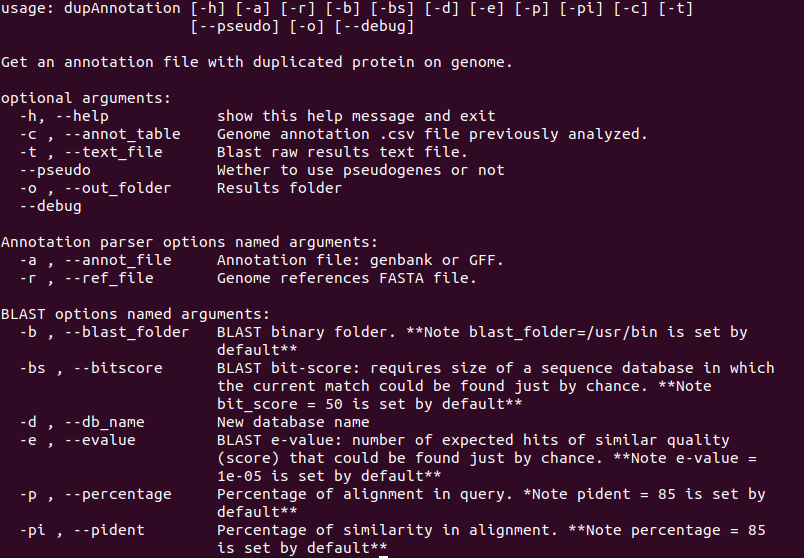
\includegraphics[width=0.7\textwidth]{figs/usage_dup_annot.png}
    \caption[Información de dup\_annot en la terminal]{Información del uso de argumentos de dup\_annot}
    \label{fig:usage_dup_annot}
\end{figure}



Además de los argumentos incluidos en los módulos anteriores, añadimos uno nuevo que permitirá elegir si se quiere tener en cuenta los pseudogenes o no en el resultado final.

El módulo dup\_annot.py toma los resultados en bruto de BLAST e identifica los diferentes grupos de duplicados, teniendo en cuenta que si A=B y B=C, entonces A=B=C. Esta nueva información la volcará en la tabla de anotación generada en input\_parser (o proporcionada por el usuario), de la cual se mantendrán únicamente las proteínas duplicadas.  De esta forma, obtenemos una tabla de anotación completa para cada una de las proteínas duplicadas, identificadas por el grupo de duplicado al que pertenecen.

Al finalizar el proceso, el programa muestra en pantalla cuántos grupos y proteínas duplicadas ha encontrado con los parámetros de BLAST introducidos (figura \ref{fig:salida_dup_annot})

\begin{figure}[h]
	\centering
	\captionsetup{width=0.7\linewidth} 
	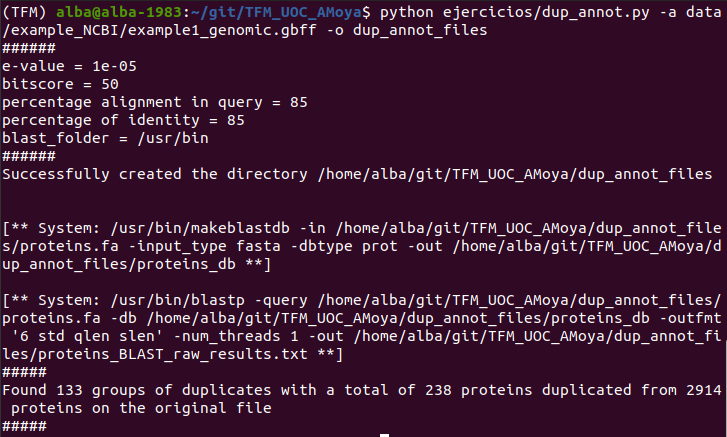
\includegraphics[width=0.7\linewidth]{figs/salida_dup_annot.png}
	\caption[Mensaje terminal de dup\_annot.py]{Mensaje mostrado en la terminal de Linux al terminar el proceso de dup\_annot.py.}
	\label{fig:salida_dup_annot}
\end{figure}

\subsection{Archivos obtenidos} 

Como muestra la figura (\ref{fig:salida_dup_annot}) al final del proceso obtenemos una carpeta con todos los archivos generados juntos.

\begin{figure}[h]
	\centering
	\captionsetup{width=0.4\linewidth} 
	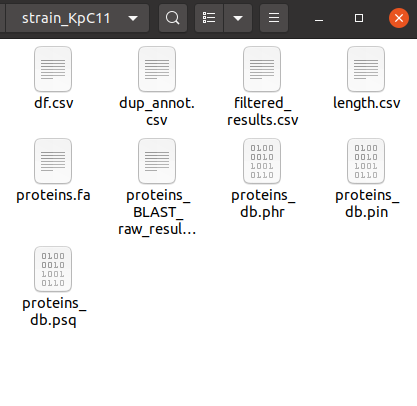
\includegraphics[width=0.4\linewidth]{figs/input_parser_files.png}
	\caption[Carpeta de resultados]{Carpeta de resultados generada tras ejecutar el programa dup\_annot.py}
	\label{fig:salida_dup_annot}
\end{figure}

- Del tratamiento de datos con input\_parser se obtienen los archivos df.csv (tabla de anotación completa), proteins.fa (secuencias de proteínas) y length.csv (longitudes de los diferentes genomas contenidos).

- La búsqueda de resultados con dup\_searcher nos proporciona los archivos pertenecientes a la base de datos creada (proteins\_db), el archivo proteins\_BLAST\_raw\_resuts.txt con los alineamientos generados y filtered\_results.csv tras pasar por el proceso de filtrado de los mejores resultados.

- Finalmente, dup\_annot.csv es la tabla de anotación para las proteínas identificadas como duplicados.

\section{Módulo en $\mathbb{R}$}

Se ha utilizado la versión 4.0.3 de R, en el entorno de desarrollo RStudio (versión 1.3.1073). Se ha creado un proyecto específico para desarrollar el paquete cuyas especificaciones se detallan en el apéndice \ref{apA}.

Se ha utilizado el paquete \textbf{BioCircos} \cite{cui_biocircosjs_2016, vulliard_biocircos_2019} para generar gráficos circulares que representen el cromosoma bacteriano y sus posibles plásmidos, resaltando los genes duplicados y sus grupos localizados en la primera fase del proyecto. En la figura \ref{fig:ex_BioCircos} se puede ver un ejemplo de gráfico generado con BioCircos.

\begin{figure}[h]
	\centering
	\captionsetup{width=0.5\linewidth} 
	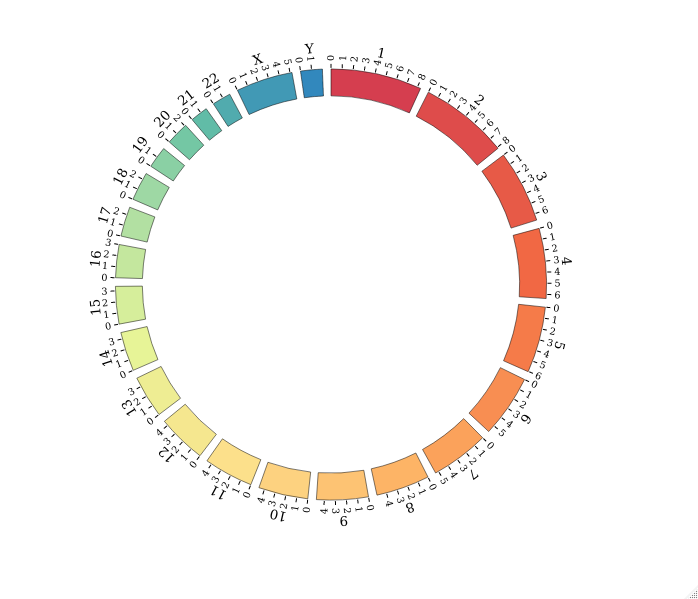
\includegraphics[width=0.5\linewidth]{figs/ex_biocircos.png}
	\caption[Ejemplo de gráfico BioCircos]{Gráfico generado automáticamente con los datos por defecto del paquete BioCircos de R. Se pueden ver los diferentes cromosomas del genoma humano identificados por colores y con un tamaño proporcional con respecto a la totalidad del genoma.}
	\label{fig:ex_BioCircos}
\end{figure}

A continuación se hará una breve descripción de las funciones más significativas del módulo. 

\begin{itemize}
    \item \textbf{duplicate\_group\_tracks:} para cada grupo de duplicados se determinará el cromosoma o plásmido a los que pertenecen sus componentes (rec\_id), posición e inicio de cada secuencia. Se generará un \textit{track} en el que las secuencias duplicadas se conectaran con líneas con los miembros de su grupo de duplicación.
    \item \textbf{parse\_data}: genera la información que se mostrará al pasar el cursor del ratón por encima de cada secuencia duplicada y la paleta de colores que identificará cada tipo de información.
    \item \textbf{add\_genes\_strand:} para cada hebra del cromosoma, se creará un círculo o track donde se podrán ver los genes duplicados alojados.
    \item \textbf{create\_BioCircos:} finalmente se crea el gráfico con la información generada en las funciones previas.
\end{itemize}

%% añade un ejemplo bonito de biocircos con tus datos y lo comentas brevemente sin entrar en detalle de los resultados.
\chapter{Análisis de duplicaciones génicas en una selección de cepas bacterianas}
\label{chapter: analisis}

%% reorganizado
Con el fin de complementar la caracterización de duplicidades en cepas de \textit{E. coli} y diferentes especies de estafilococos y enterococos descritas anteriormente \cite{bernabeu_gene_2019, sanchez-herrero_gene_2020} y como ejemplo de uso de las herramientas desarrolladas durante este TFM descritas en el capítulo \ref{chapter: desarrollo} se ha hecho un análisis de la duplicación génica en cepas bacterianas del grupo ESKAPE. Se han utilizado las especies del grupo no incluidas en estos trabajos (\textbf{\textit{Klebsiella pneumoniae, Acinetobacter baumannii, Pseudomonas aeruginosa, Enterobacter} spp.}.

Este grupo de bacterias se caracteriza por ser especialmente patógenas al presentar resistencia a los antibióticos conocidos para el tratamiento de las enfermedades derivadas de ellas \cite{pendleton_clinical_2013, chavez-jacobo_batalla_2020}. Son bacterias Gram-negativas de marcado comportamiento oportunista que colonizan las vías respiratorias y digestivas de individuos inmunodeprimidos provocando infecciones y neumonías graves. Al ser muy resistentes a los antibióticos conocidos su tratamiento puede complicarse llegando a la muerte del paciente \cite{toro_klebsiella_2010, farinas_infecciones_2013, todar_pseudomonas_nodate, dworkin_genus_2006}. 

\section{Selección de cepas}

Para realizar la selección de cepas a analizar, se ha procedido a realizar una búsqueda en la base de datos de genomas del NCBI \cite{noauthor_home_nodate} para cada una de las especies a estudio. Se han filtrado los resultados para obtener genomas completos y patógenas para el ser humano, los resultados obtenidos se ordenaron por fecha de actualización y se eligieron las cuatro cepas más actuales de cada especie (figura \ref{fig:busqueda_ncbi}). En la tabla \ref{table:cepas} se muestran las cepas seleccionadas.

\begin{figure}
	\centering
	\captionsetup{width=\linewidth} 
	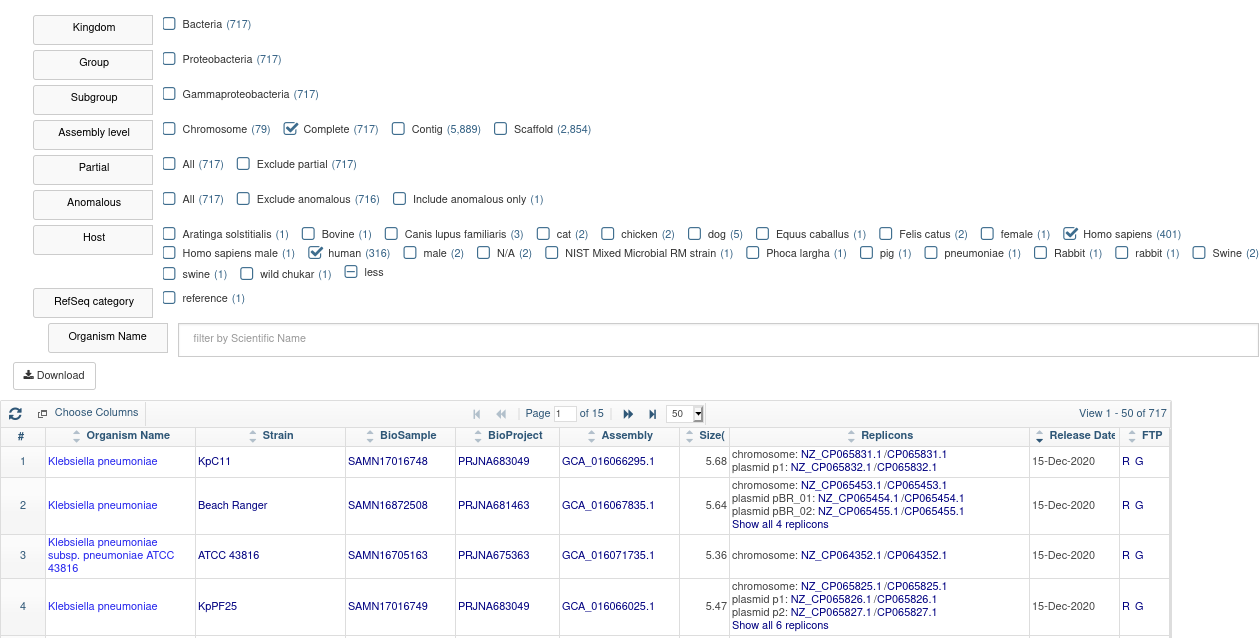
\includegraphics[width=\linewidth]{figs/busqueda_ncbi.png}
	\caption[Filtro de resultados de NCBI]{Resultados obtenidos en NCBI al hacer una búsqueda de la cepa de interés y aplicar los filtros deseados. Los resultados se han ordenado por fecha de actualizaciónn para poder seleccionar las cepas con los datos más actualizados.}
	\label{fig:busqueda_ncbi}
\end{figure}

\begin{table}
	\centering
	\captionsetup{width=0.5\linewidth}
	\begin{tabular}{ l || c }
		\hline
		Especie & Cepa\\
		\hline
		\hline
		\multirow{4}{*}{\textit{Klebsiella pneumoniae}} & KpC11 \\
		%\hline
		& ATCC 43816 \\
		%\hline
		& Beach Ranger \\
		%\hline
		& KpPF25 \\
		\hline
		\multirow{4}{*}{\textit{Acinetobacter baumannii}} & ATCC 17961 \\
		%\hline
		& TP3 \\
		%\hline
		& TP2 \\
		%\hline
		& FDAARGOS\_1036 \\
		\hline
		\multirow{4}{*}{\textit{Pseudomonas aeruginosa}} & DL201330 \\
		%\hline
		& TJ2014-049 \\
		%\hline
		& TJ2019-017 \\
		%\hline
		& TJ2019-022 \\
		\hline
		\multirow{4}{*}{\textit{Enterobacter cloacae}} & STN0717-73  \\
		& STN0717-60  \\
		& RHBSTW-00399  \\
		& RHBSTW-00490  \\
		\hline
	\end{tabular}
	\caption{Cepas seleccionadas para llevar a cabo la búsqueda de duplicidades y ejemplo de uso de la herramienta.}
	\label{table:cepas}
\end{table}


\newpage
\section{Búsqueda y representación de duplicidades}

A continuación se muestra como ejemplo de uso de las herramientas desarrolladas en la búsqueda, anotación y representación de duplicidades génicas de la cepa Beach Ranger de \textit{Klebsiella pneumoniae}. El motivo de la elección de esta cepa como muestra de ejemplo es meramente didáctico. Es un grupo de bacterias con varios plásmidos de diferentes tamaños y muestra duplicidades tanto en las hebras positivas como negativas. Estas características se prestan a generar unas gráficas visualmente atractivas y completas para explicar cada uno de los elementos que nos encontramos.

\paragraph{\textbf{- Datos: }} Los archivos de anotación completos se pueden descargar directamente del servidor de búsqueda del NCBI, accediendo a la carpeta ftp del servidor (figura \ref{fig:ncbi_beach}) desde el link que se ofrece en la columna correspondiente. Si se desea el genoma del cromosoma o un plásmido en concreto, se puede acceder a ellos directamente desde los enlaces de la tabla de resultados de búsqueda.

\begin{figure}[h]
	\centering
	\captionsetup{width=0.6\linewidth} 
	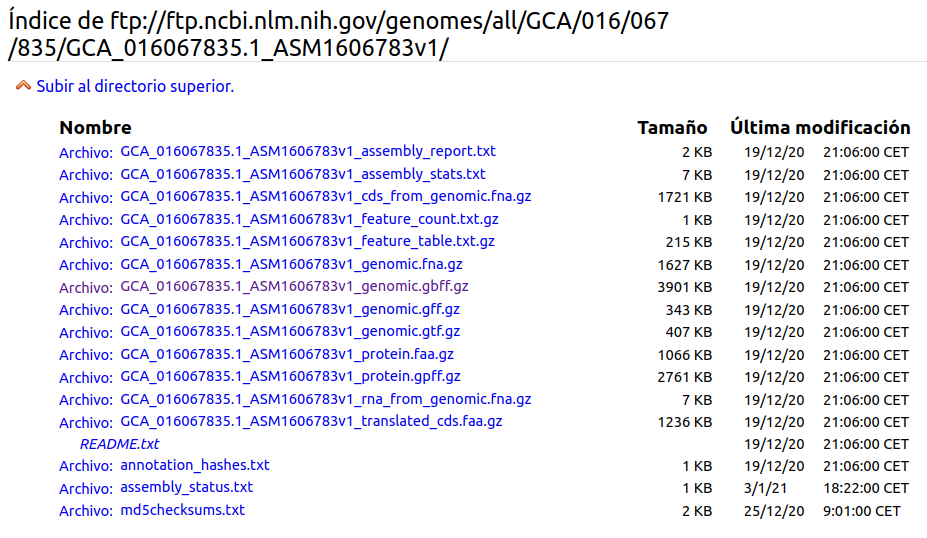
\includegraphics[width=0.6\linewidth]{figs/ncbi_beach.png}
	\caption[Carpeta ftp de NCBI]{Contenido de archivos de la carpeta correspondiente a la cepa Beach Ranger del servidor ftp de NCBI}
	\label{fig:ncbi_beach}
\end{figure}

Hemos seleccionado la anotación en formato \textit{GenBank} (extensión gbff) ya que nos permite utilizar un único documento, favoreciendo la agilidad del proceso.

\paragraph{\textbf{- Búsqueda y anotación de duplicados: }} Siguiendo las indicaciones dadas en el capítulo anterior. Invocamos desde la terminal el módulo dup\_annot.py y aportamos la información conveniente. Dejamos los valores de los parámetros que se dan por defecto y generamos los resultados (figura \ref{fig:ex_beach}).

\begin{figure}[h]
	\centering
	\captionsetup{width=0.7\linewidth} 
	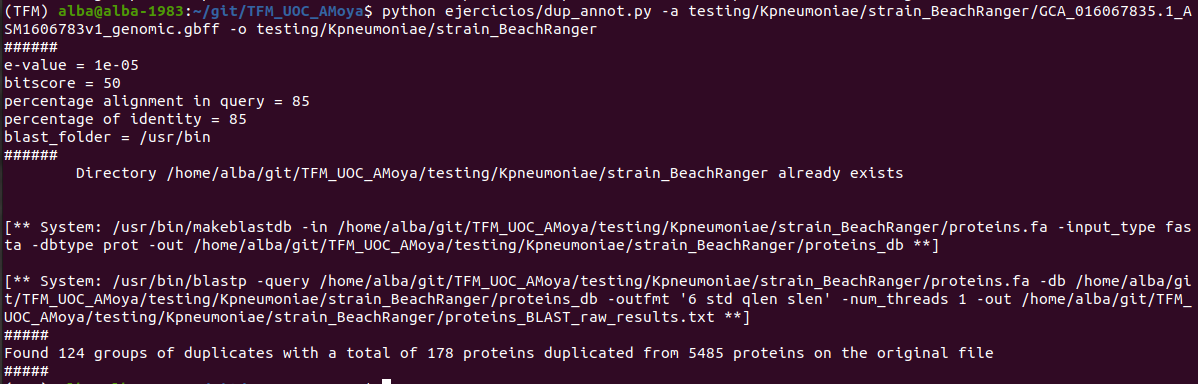
\includegraphics[width=0.7\linewidth]{figs/ex_beach.png}
	\caption[Ejemplo de uso en la cepa Beach Ranger]{Resultados obtenidos en la terminal al invocar dup\_annot.py con los datos para la cepa Beach Ranger.}
	\label{fig:ex_beach}
\end{figure}

\newpage
\paragraph{\textbf{- Resultados obtenidos: }} La figura \ref{fig:beach_result} muestra un fragmento de la tabla de anotación para esas 178 proteínas duplicadas en la cepa Beach Ranger.

\begin{figure}[h]
	\centering
	\captionsetup{width=\linewidth} 
	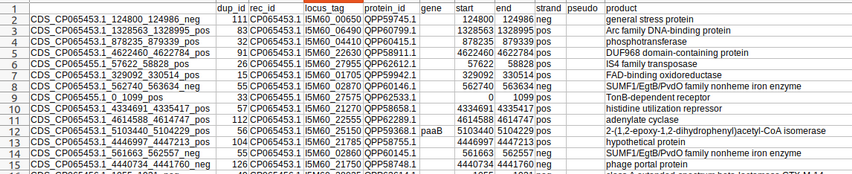
\includegraphics[width=\linewidth]{figs/beach_result.png}
	\caption[Tabla de anotación del genoma duplicado de la cepa Beach Ranger]{Tabla de anotación de las proteínas duplicadas generada tras el tratamiento de los datos de la cepa Beach Rangercon input\_parser.py}
	\label{fig:beach_result}
\end{figure}

En el apéndice \ref{apB} se puede encontrar los resultados obtenidos para la totalidad de las cepas estudiadas.

\paragraph{\textbf{- Representación gráfica: }} Finamente, utilizando los comandos de R procedemos a generar la gráfica que nos mostrará la distribución de las proteínas duplicadas. 

Le indicamos al programa cuáles son los datos que debe utilizar con las siguientes instrucciones: 

\vspace{5mm}
\begin{lstlisting}[language=R]
## strain BeachRanger
seq_lengths_BeachRanger <- read.csv(paste0(data_folder, "Kpneumoniae/strain_BeachRanger/length.csv"),
                                  header=FALSE, row.names=1)
bed_info_file_BeachRanger <- read.table(paste0(data_folder, "Kpneumoniae/strain_BeachRanger/dup_annot.csv"), sep=",",
                                      header=TRUE)
bed_info_file_BeachRanger <- bed_info_file_BeachRanger[,c("dup_id", "rec_id", "start", "end", "locus_tag", "product", "strand")]
\end{lstlisting}
\vspace{5mm}

Se debe considerar que el valor por defecto para los pseudogenes en dup\_annot es no tenerlos en cuenta a la hora de generar la tabla final, pero sí que se incluyeron en los grupos de duplicados correspondiente. Esto puede resultar en que nos queden grupos de duplicados con una única proteína, lo que nos generará problemas a la hora de intentar graficar los resultados. Para evitar esto, eliminamos esas proteínas huérfanas con el siguiente comando:

\vspace{5mm}
\begin{lstlisting}[language=R]
# # keep only real duplicated groups
bed_info_file_BeachRanger <- bed_info_file_BeachRanger %>% group_by(dup_id) %>% filter(n() >1)
# 
\end{lstlisting}
\vspace{5mm}

Finalmente, creamos nuestro BioCircos (figura \ref{fig:biobeach}):

\vspace{5mm}
\begin{lstlisting}[language=R]
create_BioCircos(seq_lengths = seq_lengths_BeachRanger,
                 bed_info_file = bed_info_file_BeachRanger)
\end{lstlisting}
\vspace{5mm}

\begin{figure}[h]
	\centering
	\captionsetup{width=\linewidth} 
	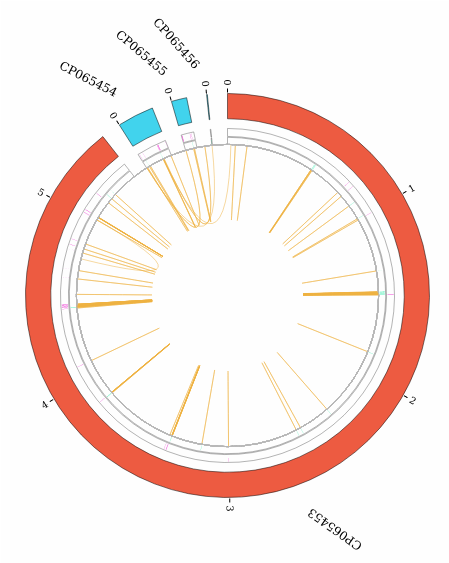
\includegraphics[width=\linewidth]{figs/biocircos_BeachRanger.png}
	\caption[Gráfica biocircos para la cepa Beach Ranger de \textit{K. pneumoniae}]{Representación gráfica con BioCircos de los genes duplicados en el genoma de la cepa Beach Ranger de \textit{K. pneumoniae}. El cromosoma de la bacteria (rojo) y sus plásmidos (azul) se representan en un mapa circular que muestra la localización de cada gen duplicado. Las siguientes dos capas muestran los genes en la hebra positiva (rosa) y negativa (turquesa). Las líneas naranja interiores señalan las conexiones entre proteínas pertenecientes al mismo grupo de duplicados. Escala de tamaño en Mb}
	\label{fig:biobeach}
\end{figure}

En el apéndice \ref{apB} se adjunta los cuatro gráficos correspondientes a cada cepa de \textit{K pneumoniae} seleccionada con objetivo comparativo. También se aporta el enlace a la carpeta github correspondiente donde encontrar todas las gráficas de las cepas analizadas y los archivos generados tras su análisis.
%% \cleardoublepage
\pagenumbering{arabic}
\setcounter{page}{1} 


\chapter{Introducción}
\label{chapter:introduccion}

\section{Contexto y justificación del trabajo}

Durante el desarrollo de este trabajo de fin de máster (TFM) se ha llevado a cabo una caracterización de las posibles duplicidades génicas presentes en los genomas de diferentes cepas bacterianas entre las especies del grupo ESKAPE no analizadas en estudios previos \textit{(Klebsiella pneumoniae, Acinetobacter baumannii, Pseudomonas aeruginosa} y  \textit{Enterobacter} spp.). Para ello se implementarán diversos módulos y paquetes específicos en los lenguajes de programación Python y R que realizarán de manera automática la búsqueda de las mismas. Con los resultados de la obtenidos, se podrán caracterizar genes específicos relacionados con virulencia o resistencia a antimicrobianos y generar gráficas para su visualización.

La duplicación genética es un proceso que se encuentra tanto en células eucariotas como procariotas y es uno de los tipos de mutación más frecuentes \cite{serres_evolution_2009,zhang_evolution_2003}. Es un mecanismo que genera una o más copias indistinguibles del mismo gen en el genoma celular y que se mantiene a lo largo de la línea evolutiva \cite{lynch_genome-wide_2008, lipinski_high_2011, sanchez-herrero_gene_2020, zhang_evolution_2003}. La ventaja evolutiva que proporciona para las bacterias mantener en sus genomas diferentes copias para el mismo gen viene determinada por que cada una de ellas podría mostrar diferentes patrones de expresión e, incluso, responder ante estímulos diferentes, lo cual dota a las cepas que portan esta variedad de copias de más oportunidades para adaptarse a variaciones fisicoquímicas del medio en el que se encuentran. El aumento de la complejidad genómica que genera esta diversidad funcional, facilita la proliferación de las células ante medios limitantes e incrementa las probabilidades de nuevas mutaciones adaptativas \cite{serres_evolution_2009,zhang_evolution_2003}.

Las bacterias del grupo ESKAPE son especialmente patógenas para los seres humanos ya que presentan en su material genético genes de resistencia a diferentes agentes antimicrobianos, lo que las hace difíciles de combatir en caso de infección \cite{lipinski_high_2011, santajit_mechanisms_2016}. La existencia de cepas patógenas multirresistentes a diferentes antibióticos ha supuesto un problema sanitario que lleva a graves consecuencias en la salud pública \cite{bernabeu_gene_2019,murray_vancomycin-resistant_2000, pendleton_clinical_2013, sanchez-herrero_gene_2020}. La limitación de los grupos científicos para crear nuevos antibióticos efectivos y la rapidez con que estas bacterias evolucionan, hace necesario aumentar los conocimientos alrededor de cómo se interrelacionan los diferentes genes bacterianos al expresarse y favorecer la supervivencia de la bacteria \cite{bernabeu_gene_2019,pendleton_clinical_2013,santajit_mechanisms_2016}.

El estudio de duplicidades génicas en \textit{E. coli}, estafilococos y enterococos ha demostrado un patrón diferenciado de las mismas entre las cepas más virulentas y las que no presentan patogenicidad. Se ha constatado la presencia de un número significativo de genes duplicados en cepas patógenas, respecto a aquellas no patógenas, que no se muestran en cepas inofensivas, lo que sugiere que estos genes podrían favorecer de forma relevante la virulencia de las mismas \cite{bernabeu_gene_2019,sanchez-herrero_gene_2020}.

La duplicación genética en bacterias se produce más frecuentemente por transferencia horizontal genética (HGT) entre diferentes individuos gracias a agentes virales, plásmidos o transposones, que por diferentes mecanismos moleculares naturales que pueden generar duplicaciones en los genomas bacterianos \cite{reams_mechanisms_2015,romero_gene_1997,sanchez-herrero_gene_2020,santajit_mechanisms_2016}. 

Identificar genes duplicados específicos en diferentes cepas patógenas, podría contribuir al estudio de los mecanismos de la virulencia de las mismas ampliando la información ya conocida sobre cómo se regula la expresión genética en las bacterias a estudio \cite{bernabeu_gene_2019,sanchez-herrero_gene_2020}. Por otro lado, si se determinara la codificación por parte de alguno de estos genes duplicados de productos antigénicos, se podrían desarrollar nuevas vacunas o medicamentos más efectivos para hacer frente a las enfermedades provocadas por este tipo de bacterias \cite{bernabeu_gene_2019, serres_evolution_2009}.

Por todo lo mencionado, en este Trabajo de TFM se complementarán los trabajos realizados por \cite{bernabeu_gene_2019} y \cite{sanchez-herrero_gene_2020} desarrollando una herramienta bioinformática capaz de llevar a cabo de manera automatizada todo el proceso de búsqueda e identificación de duplicidades dentro de un genoma dado. Se obtendría como resultado un archivo de datos con toda la información obtenida y una representación gráfica con el fin de facilitar su estudio y comprensión. Estos resultado podrán utilizarse facilmente en estudios de investigación relacionados.

Desarrollar una herramienta bioinformática, compuesta de diversos módulos específicos para cada una de las fases que comprenden el análisis genómico y la búsqueda de duplicidades, permitirá a la comunidad científica avanzar de forma más ágil en la investigación sobre el tema.



\section{Objetivos del Trabajo}

Los objetivos desarrollados a lo largo de este TFM han sido los siguientes:
\begin{itemize}
    \item Desarrollo de herramientas bioinformáticas para el análisis y caracterización de duplicidades genéticas en bacterias.
    \begin{itemize}
        \item Desarrollar funciones de python para el tratamiento y análisis de duplicaciones tanto de secuencias genómicas en bases de datos como ensambladas \textit{de novo} por parte del usuario.
        \item Implementar la generación y representación de resultados para la mejor interpretación y visualización de los datos.
    \end{itemize}
    \item Caracterización de duplicaciones génicas en una selección de cepas bacterianas.
    \begin{itemize}
        \item Selección de cepas del grupo ESKAPE para caracterizar duplicaciones génicas.
        \item Analizar las secuencias genómicas de las cepas seleccionadas y localizar e identificar genes duplicados
    \end{itemize}
\end{itemize}

\section{Enfoque y método seguido}
% Indicar cuáles son las posibles estrategias para llevar a cabo el trabajo e indicar cuál es la estrategia elegida (desarrollar un producto nuevo, adaptar un producto existente, …). Valorar porque esta es la estrategia más apropiada para conseguir los objetivos
A pesar de que ya existen trabajos previos en los cuales se muestran técnicas para el análisis de duplicidades génicas \cite{bernabeu_gene_2019, sanchez-herrero_gene_2020}, estos no presentan un desarrollo de herramientas bioinformáticas que permitan automatizar totalmente el proceso de análisis y posterior interpretación de los resultados. La estrategia que se llevará a cabo en este TFM procurará una única metodología de análisis genómico que permita a la comunidad científica realizar este proceso de una forma más directa. Cada fase del análisis, desde la lectura de los datos hasta la visualización e interpretación de resultados, se englobará en un único proceso, lo que facilitará el uso y difusión de las herramientas generadas.

En primer lugar, se han desarrollado módulos en Python \cite{Rossum_2009} para leer de manera automática la secuencia genómica proporcionada por el usuario y analizar la información indicada. Posteriormente, con la herramienta de análisis de secuencias BLAST+ \cite{madden_blast_2003}, se ha implementado otros módulos para buscar e identificar genes duplicados y generar un archivo de resultados. Los diferentes módulos creados en python se han integrado en una única herramienta que trabajará de manera automática a lo largo de todos los pasos requeridos para completar el análisis.

Finalmente, se ha creado un paquete en R \cite{R_core} para mostrar los resultados de manera interactiva con el programa BioCircos \cite{biocircos} que facilitan su interpretación. Este módulo se ha generado a partir del aportado por \cite{sanchez-herrero_gene_2020} con las modificaciones pertinentes para adaptarlo a nuestras necesidades.

Una vez desarrollada esta versión beta del programa, se ha desarrollado el segundo objetivo y analizado cepas bacterianas reales para generar resultados.


\section{Planificación del Trabajo}

% Descripción de los recursos necesarios para realizar el trabajo, las tareas a realizar y una planificación temporal de cada tarea utilizando un diagrama de Gantt o similar. Esta planificación tendría que marcar cuáles son los hitos parciales de cada una de las PEC.

Los objetivos y tareas realizados se han planteado según los diferentes hitos marcados por el plan docente. Estos hitos corresponden a cada una de las pruebas de evaluación continua (PEC) propuestas a lo largo del periodo estipulado, así como la entrega de la memoria final y la defensa pública del proyecto por medio de una presentación virtual.

La imagen \ref{fig:crono} representa la planificación del TFM. Se ha desglosado cada objetivo en las correspondientes tareas a realizar a lo largo de la línea temporal.

\begin{figure}[h]
	\centering
	\captionsetup{width=0.7\linewidth} 
	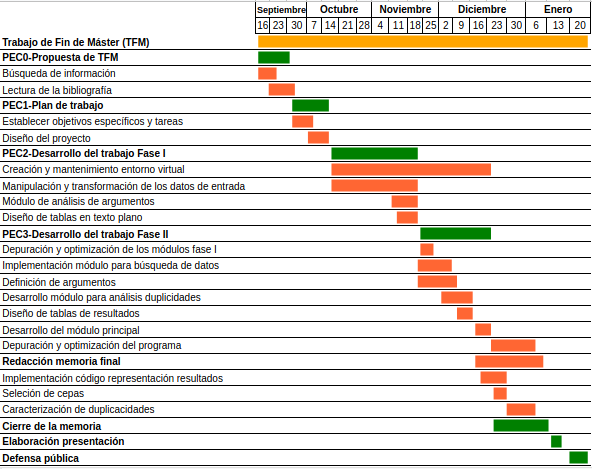
\includegraphics[width=0.7\linewidth]{figs/cronograma.png}
	\caption[Cronograma]{Cronograma detallado de la planificación del trabajo a lo largo de desarrollo del TFM. En verde se representan las entregas de documentación y en naranja las diferentes tareas realizadas.}
	\label{fig:crono}
\end{figure}
A continuación, se presenta un breve resumen de algunas de las tareas realizadas más significativas:

\begin{itemize}
    \item \textbf{Creación de un entorno virtual en Python: }para poder realizar correctamente las tareas de programación, se ha creado un espacio único para el proyecto en el que se albergue las diferentes librerías instaladas. El manejo del programa de instalación \textit{pip} ha sido fundamental para el desarrollo de este entorno. Así como el uso de aplicaciones para el control de versiones como GIT y el trabajo colaborativo en plataformas virtuales como GitHub ha favorecido la fluidez a la hora de realizar correcciones y sugerencias por parte del director de TFM y la comunicación entre ambas partes.
    
    \item \textbf{Desarrollo de módulos básicos: }Se han creado las diferentes funciones necesarias para implementar el módulo para la búsqueda de datos. Estos módulos básicos se han concebido como pequeños fragmentos de código funcionales capaces de realizar las diferentes acciones de manipulación y transformación de los datos proporcionados. De esta forma, se obtendrán objetos que puedan ser utilizados en el módulo principal. Se han utilizado herramientas en BioPython profundizando en la documentación proporcionada para cada función y adaptándolas a nuestras necesidades para la creación de los nuevos programas.
    
    \item \textbf{Transformación de la información a texto plano: }mediante los programas Pandas y Numpy, se han manipulado los archivos de anotación genómicos (e.g. genbank, GTF, GFF) para crear objetos de python con la estructura adecuada para generar tablas y poder volcarlas como texto plano y visualizarlas, por ejemplo, en un procesador de hojas de cálculo. Estas tablas se han utilizado posteriormente para analizar las duplicidades génicas de los genomas estudiados.
    
    \item \textbf{Depuración de los módulos creados: }durante la primera fase del proyecto, se generaron una serie de módulos que debían ser depurados para su correcto funcionamiento. El seguimiento de errores de programación y su resolución han llevado un tiempo necesario para que el funcionamiento de los siguientes módulos asociados fuera correcto. Se ha implementado el programa de forma que sea muy flexible en cuanto al tipo de información proporcionada por el usuario.
    
    \item \textbf{Definición de argumentos: }para desarrollar una herramienta versátil y de fácil manejo por parte del usuario, se debe ofrecer un amplio rango de posibilidades que faciliten su uso sea cuál sea el tipo de archivo que se utilice para la búsqueda de duplicidades. Así, se han previsto distintos escenarios para definir los argumentos posibles y generar los resultados en una única línea de comandos en la consola LINUX.
    
    \item \textbf{Diseño de tablas de resultados: }mediante los programas Pandas y Numpy se han definido los archivos de texto plano para formatear las tablas con los resultados obtenidos.
    
    \item \textbf{Desarrollo del módulo principal: }Para posibilitar la búsqueda de duplicidades en solo una línea de comando en la terminal, todos los módulos programados previamente deben relacionarse entre sí para poder funcionar como un conjunto. Este módulo principal recogerá los argumentos proporcionados por el usuario y, en base a ello, utilizará unas funciones u otras para generar el archivo de resultados.
    
    \item \textbf{Implementación del código para la representación de resultados: }Implementación del módulo en R que permitirá representar los resultados. Con el paquete BioCircos se ha diseñado un script adaptado a las peculiaridades de los datos generados por el programa en python para generar gráficos representativos del genoma estudiado y los diferentes grupos de duplicados relacionados entre sí.
\end{itemize}












\section{Breve sumario de productos obtenidos}
% No hay que entrar en detalle: la descripción detallada se hará en el resto de capítulos. 

Durante el periodo de realización del TFM se han entregado los siguientes documentos:

\begin{itemize}
    \item Propuesta de TFM.
    \item Pruebas de evaluación contínua:
    \begin{itemize}
        \item Definición de los contenidos del trabajo.
        \item Plan de trabajo.
        \item Informes de seguimiento
    \end{itemize}
\end{itemize}

A estos documentos, se deben añadir la presente memoria y la presentación y defensa del TFM. Finalmente, se realizará un informe de autoevaluación que también será entregado con el resto de documentación.

Además de estos documentos, se han obtenido los siguientes productos:

\begin{itemize}
    \item Secuencias de comandos (scripts) de los módulos en python.
    \item Script del programa en R.
    \item Tablas de anotación y gráficos de las duplicidades génicas de las cepas seleccionadas.
    \item Repositorio público en github con todos los scripts desarrollados, documentación y resultados generados. ******incluir link cuando esté todo listo****
\end{itemize}

\section{Breve descripción de los otros capítulos de la memoria}
El capítulo \ref{chapter: desarrollo} se ha dedicado a explicar detalladamente cada módulo desarrollado y su funcionamiento. Cada una de las secciones del capítulo corresponde a las diferentes fases del proceso, desde la entrada de datos hasta la generación de resultados y su representación gráfica.

El capítulo \ref{chapter: analisis} describe el uso de las herramientas creadas para el análisis de duplicidades en cepas bacterianas seleccionadas. 

El apédice \ref{apA} contiene información sobre los requerimientos necesarios para utilizar los módulos implementados. Se resume brevemente los programas complementarios que se deben instalar y los enlaces al repositorio en github para la descarga de los scripts completos.

Por último, el apéndice \ref{apB} incluye los resultados obtenidos en el análisis de las cepas seleccionadas.
%% \cleardoublepage
\pagenumbering{arabic}
\setcounter{page}{1} 


\chapter{Introducción}
\label{chapter:introduccion}

\section{Contexto y justificación del trabajo}

Durante el desarrollo de este trabajo de fin de máster (TFM) se ha llevado a cabo una caracterización de las posibles duplicidades génicas presentes en los genomas de diferentes cepas bacterianas entre las especies del grupo ESKAPE no analizadas en estudios previos \textit{(Klebsiella pneumoniae, Acinetobacter baumannii, Pseudomonas aeruginosa} y  \textit{Enterobacter} spp.). Para ello se implementarán diversos módulos y paquetes específicos en los lenguajes de programación Python y R que realizarán de manera automática la búsqueda de las mismas. Con los resultados de la obtenidos, se podrán caracterizar genes específicos relacionados con virulencia o resistencia a antimicrobianos y generar gráficas para su visualización.

La duplicación genética es un proceso que se encuentra tanto en células eucariotas como procariotas y es uno de los tipos de mutación más frecuentes \cite{serres_evolution_2009,zhang_evolution_2003}. Es un mecanismo que genera una o más copias indistinguibles del mismo gen en el genoma celular y que se mantiene a lo largo de la línea evolutiva \cite{lynch_genome-wide_2008, lipinski_high_2011, sanchez-herrero_gene_2020, zhang_evolution_2003}. La ventaja evolutiva que proporciona para las bacterias mantener en sus genomas diferentes copias para el mismo gen viene determinada por que cada una de ellas podría mostrar diferentes patrones de expresión e, incluso, responder ante estímulos diferentes, lo cual dota a las cepas que portan esta variedad de copias de más oportunidades para adaptarse a variaciones fisicoquímicas del medio en el que se encuentran. El aumento de la complejidad genómica que genera esta diversidad funcional, facilita la proliferación de las células ante medios limitantes e incrementa las probabilidades de nuevas mutaciones adaptativas \cite{serres_evolution_2009,zhang_evolution_2003}.

Las bacterias del grupo ESKAPE son especialmente patógenas para los seres humanos ya que presentan en su material genético genes de resistencia a diferentes agentes antimicrobianos, lo que las hace difíciles de combatir en caso de infección \cite{lipinski_high_2011, santajit_mechanisms_2016}. La existencia de cepas patógenas multirresistentes a diferentes antibióticos ha supuesto un problema sanitario que lleva a graves consecuencias en la salud pública \cite{bernabeu_gene_2019,murray_vancomycin-resistant_2000, pendleton_clinical_2013, sanchez-herrero_gene_2020}. La limitación de los grupos científicos para crear nuevos antibióticos efectivos y la rapidez con que estas bacterias evolucionan, hace necesario aumentar los conocimientos alrededor de cómo se interrelacionan los diferentes genes bacterianos al expresarse y favorecer la supervivencia de la bacteria \cite{bernabeu_gene_2019,pendleton_clinical_2013,santajit_mechanisms_2016}.

El estudio de duplicidades génicas en \textit{E. coli}, estafilococos y enterococos ha demostrado un patrón diferenciado de las mismas entre las cepas más virulentas y las que no presentan patogenicidad. Se ha constatado la presencia de un número significativo de genes duplicados en cepas patógenas, respecto a aquellas no patógenas, que no se muestran en cepas inofensivas, lo que sugiere que estos genes podrían favorecer de forma relevante la virulencia de las mismas \cite{bernabeu_gene_2019,sanchez-herrero_gene_2020}.

La duplicación genética en bacterias se produce más frecuentemente por transferencia horizontal genética (HGT) entre diferentes individuos gracias a agentes virales, plásmidos o transposones, que por diferentes mecanismos moleculares naturales que pueden generar duplicaciones en los genomas bacterianos \cite{reams_mechanisms_2015,romero_gene_1997,sanchez-herrero_gene_2020,santajit_mechanisms_2016}. 

Identificar genes duplicados específicos en diferentes cepas patógenas, podría contribuir al estudio de los mecanismos de la virulencia de las mismas ampliando la información ya conocida sobre cómo se regula la expresión genética en las bacterias a estudio \cite{bernabeu_gene_2019,sanchez-herrero_gene_2020}. Por otro lado, si se determinara la codificación por parte de alguno de estos genes duplicados de productos antigénicos, se podrían desarrollar nuevas vacunas o medicamentos más efectivos para hacer frente a las enfermedades provocadas por este tipo de bacterias \cite{bernabeu_gene_2019, serres_evolution_2009}.

Por todo lo mencionado, en este Trabajo de TFM se complementarán los trabajos realizados por \cite{bernabeu_gene_2019} y \cite{sanchez-herrero_gene_2020} desarrollando una herramienta bioinformática capaz de llevar a cabo de manera automatizada todo el proceso de búsqueda e identificación de duplicidades dentro de un genoma dado. Se obtendría como resultado un archivo de datos con toda la información obtenida y una representación gráfica con el fin de facilitar su estudio y comprensión. Estos resultado podrán utilizarse facilmente en estudios de investigación relacionados.

Desarrollar una herramienta bioinformática, compuesta de diversos módulos específicos para cada una de las fases que comprenden el análisis genómico y la búsqueda de duplicidades, permitirá a la comunidad científica avanzar de forma más ágil en la investigación sobre el tema.



\section{Objetivos del Trabajo}

Los objetivos desarrollados a lo largo de este TFM han sido los siguientes:
\begin{itemize}
    \item Desarrollo de herramientas bioinformáticas para el análisis y caracterización de duplicidades genéticas en bacterias.
    \begin{itemize}
        \item Desarrollar funciones de python para el tratamiento y análisis de duplicaciones tanto de secuencias genómicas en bases de datos como ensambladas \textit{de novo} por parte del usuario.
        \item Implementar la generación y representación de resultados para la mejor interpretación y visualización de los datos.
    \end{itemize}
    \item Caracterización de duplicaciones génicas en una selección de cepas bacterianas.
    \begin{itemize}
        \item Selección de cepas del grupo ESKAPE para caracterizar duplicaciones génicas.
        \item Analizar las secuencias genómicas de las cepas seleccionadas y localizar e identificar genes duplicados
    \end{itemize}
\end{itemize}

\section{Enfoque y método seguido}
% Indicar cuáles son las posibles estrategias para llevar a cabo el trabajo e indicar cuál es la estrategia elegida (desarrollar un producto nuevo, adaptar un producto existente, …). Valorar porque esta es la estrategia más apropiada para conseguir los objetivos
A pesar de que ya existen trabajos previos en los cuales se muestran técnicas para el análisis de duplicidades génicas \cite{bernabeu_gene_2019, sanchez-herrero_gene_2020}, estos no presentan un desarrollo de herramientas bioinformáticas que permitan automatizar totalmente el proceso de análisis y posterior interpretación de los resultados. La estrategia que se llevará a cabo en este TFM procurará una única metodología de análisis genómico que permita a la comunidad científica realizar este proceso de una forma más directa. Cada fase del análisis, desde la lectura de los datos hasta la visualización e interpretación de resultados, se englobará en un único proceso, lo que facilitará el uso y difusión de las herramientas generadas.

En primer lugar, se han desarrollado módulos en Python \cite{Rossum_2009} para leer de manera automática la secuencia genómica proporcionada por el usuario y analizar la información indicada. Posteriormente, con la herramienta de análisis de secuencias BLAST+ \cite{madden_blast_2003}, se ha implementado otros módulos para buscar e identificar genes duplicados y generar un archivo de resultados. Los diferentes módulos creados en python se han integrado en una única herramienta que trabajará de manera automática a lo largo de todos los pasos requeridos para completar el análisis.

Finalmente, se ha creado un paquete en R \cite{R_core} para mostrar los resultados de manera interactiva con el programa BioCircos \cite{biocircos} que facilitan su interpretación. Este módulo se ha generado a partir del aportado por \cite{sanchez-herrero_gene_2020} con las modificaciones pertinentes para adaptarlo a nuestras necesidades.

Una vez desarrollada esta versión beta del programa, se ha desarrollado el segundo objetivo y analizado cepas bacterianas reales para generar resultados.


\section{Planificación del Trabajo}

% Descripción de los recursos necesarios para realizar el trabajo, las tareas a realizar y una planificación temporal de cada tarea utilizando un diagrama de Gantt o similar. Esta planificación tendría que marcar cuáles son los hitos parciales de cada una de las PEC.

Los objetivos y tareas realizados se han planteado según los diferentes hitos marcados por el plan docente. Estos hitos corresponden a cada una de las pruebas de evaluación continua (PEC) propuestas a lo largo del periodo estipulado, así como la entrega de la memoria final y la defensa pública del proyecto por medio de una presentación virtual.

La imagen \ref{fig:crono} representa la planificación del TFM. Se ha desglosado cada objetivo en las correspondientes tareas a realizar a lo largo de la línea temporal.

\begin{figure}[h]
	\centering
	\captionsetup{width=0.7\linewidth} 
	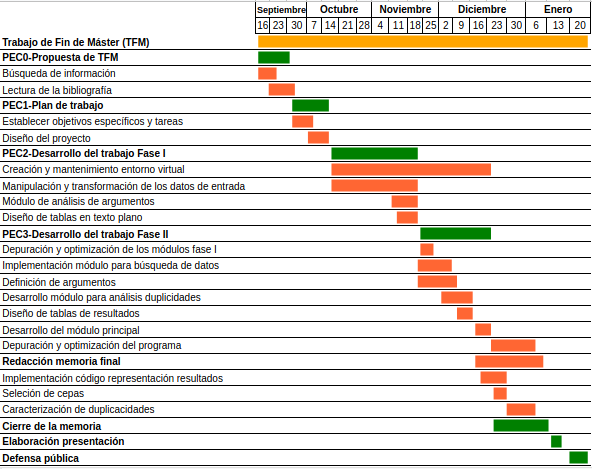
\includegraphics[width=0.7\linewidth]{figs/cronograma.png}
	\caption[Cronograma]{Cronograma detallado de la planificación del trabajo a lo largo de desarrollo del TFM. En verde se representan las entregas de documentación y en naranja las diferentes tareas realizadas.}
	\label{fig:crono}
\end{figure}
A continuación, se presenta un breve resumen de algunas de las tareas realizadas más significativas:

\begin{itemize}
    \item \textbf{Creación de un entorno virtual en Python: }para poder realizar correctamente las tareas de programación, se ha creado un espacio único para el proyecto en el que se albergue las diferentes librerías instaladas. El manejo del programa de instalación \textit{pip} ha sido fundamental para el desarrollo de este entorno. Así como el uso de aplicaciones para el control de versiones como GIT y el trabajo colaborativo en plataformas virtuales como GitHub ha favorecido la fluidez a la hora de realizar correcciones y sugerencias por parte del director de TFM y la comunicación entre ambas partes.
    
    \item \textbf{Desarrollo de módulos básicos: }Se han creado las diferentes funciones necesarias para implementar el módulo para la búsqueda de datos. Estos módulos básicos se han concebido como pequeños fragmentos de código funcionales capaces de realizar las diferentes acciones de manipulación y transformación de los datos proporcionados. De esta forma, se obtendrán objetos que puedan ser utilizados en el módulo principal. Se han utilizado herramientas en BioPython profundizando en la documentación proporcionada para cada función y adaptándolas a nuestras necesidades para la creación de los nuevos programas.
    
    \item \textbf{Transformación de la información a texto plano: }mediante los programas Pandas y Numpy, se han manipulado los archivos de anotación genómicos (e.g. genbank, GTF, GFF) para crear objetos de python con la estructura adecuada para generar tablas y poder volcarlas como texto plano y visualizarlas, por ejemplo, en un procesador de hojas de cálculo. Estas tablas se han utilizado posteriormente para analizar las duplicidades génicas de los genomas estudiados.
    
    \item \textbf{Depuración de los módulos creados: }durante la primera fase del proyecto, se generaron una serie de módulos que debían ser depurados para su correcto funcionamiento. El seguimiento de errores de programación y su resolución han llevado un tiempo necesario para que el funcionamiento de los siguientes módulos asociados fuera correcto. Se ha implementado el programa de forma que sea muy flexible en cuanto al tipo de información proporcionada por el usuario.
    
    \item \textbf{Definición de argumentos: }para desarrollar una herramienta versátil y de fácil manejo por parte del usuario, se debe ofrecer un amplio rango de posibilidades que faciliten su uso sea cuál sea el tipo de archivo que se utilice para la búsqueda de duplicidades. Así, se han previsto distintos escenarios para definir los argumentos posibles y generar los resultados en una única línea de comandos en la consola LINUX.
    
    \item \textbf{Diseño de tablas de resultados: }mediante los programas Pandas y Numpy se han definido los archivos de texto plano para formatear las tablas con los resultados obtenidos.
    
    \item \textbf{Desarrollo del módulo principal: }Para posibilitar la búsqueda de duplicidades en solo una línea de comando en la terminal, todos los módulos programados previamente deben relacionarse entre sí para poder funcionar como un conjunto. Este módulo principal recogerá los argumentos proporcionados por el usuario y, en base a ello, utilizará unas funciones u otras para generar el archivo de resultados.
    
    \item \textbf{Implementación del código para la representación de resultados: }Implementación del módulo en R que permitirá representar los resultados. Con el paquete BioCircos se ha diseñado un script adaptado a las peculiaridades de los datos generados por el programa en python para generar gráficos representativos del genoma estudiado y los diferentes grupos de duplicados relacionados entre sí.
\end{itemize}












\section{Breve sumario de productos obtenidos}
% No hay que entrar en detalle: la descripción detallada se hará en el resto de capítulos. 

Durante el periodo de realización del TFM se han entregado los siguientes documentos:

\begin{itemize}
    \item Propuesta de TFM.
    \item Pruebas de evaluación contínua:
    \begin{itemize}
        \item Definición de los contenidos del trabajo.
        \item Plan de trabajo.
        \item Informes de seguimiento
    \end{itemize}
\end{itemize}

A estos documentos, se deben añadir la presente memoria y la presentación y defensa del TFM. Finalmente, se realizará un informe de autoevaluación que también será entregado con el resto de documentación.

Además de estos documentos, se han obtenido los siguientes productos:

\begin{itemize}
    \item Secuencias de comandos (scripts) de los módulos en python.
    \item Script del programa en R.
    \item Tablas de anotación y gráficos de las duplicidades génicas de las cepas seleccionadas.
    \item Repositorio público en github con todos los scripts desarrollados, documentación y resultados generados. ******incluir link cuando esté todo listo****
\end{itemize}

\section{Breve descripción de los otros capítulos de la memoria}
El capítulo \ref{chapter: desarrollo} se ha dedicado a explicar detalladamente cada módulo desarrollado y su funcionamiento. Cada una de las secciones del capítulo corresponde a las diferentes fases del proceso, desde la entrada de datos hasta la generación de resultados y su representación gráfica.

El capítulo \ref{chapter: analisis} describe el uso de las herramientas creadas para el análisis de duplicidades en cepas bacterianas seleccionadas. 

El apédice \ref{apA} contiene información sobre los requerimientos necesarios para utilizar los módulos implementados. Se resume brevemente los programas complementarios que se deben instalar y los enlaces al repositorio en github para la descarga de los scripts completos.

Por último, el apéndice \ref{apB} incluye los resultados obtenidos en el análisis de las cepas seleccionadas.

% Conclusiones
\chapter*{Conclusiones}
\label{chapter:conclusiones}

% Este capítulo tiene que incluir:

% Una descripción de las conclusiones del trabajo: Qué lecciones se han aprendido del trabajo?.

% Una reflexión crítica sobre el logro de los objetivos planteados inicialmente: Hemos logrado todos los objetivos? Si la respuesta es negativa, por qué motivo? 

% Un análisis crítico del seguimiento de la planificación y metodología a lo largo del producto: Se ha seguido la planificación? La metodología prevista ha sido la adecuada? Ha habido que introducir cambios para garantizar el éxito del trabajo? Por qué? 

% Las líneas de trabajo futuro que no se han podido explorar en este trabajo y han quedado pendientes. 

En este proyecto se ha diseñado una línea de trabajo para la búsqueda de duplicidades genómicas a partir de ficheros de anotación proporcionados por el usuario. Para llevar a cabo el proceso, se ha desarrollado una serie de programas o módulos en python y R que automatizan el análisis de los datos. El resultado final del proceso de análisis es una tabla de anotación de las proteínas duplicadas halladas en el genoma a estudio y una representación gráfica de las mismas.

El trabajo ha supuesto un gran reto tanto en su diseño como en la depuración del código y puesta a punto de los programas debido al gran esfuerzo que supone aprender un lenguaje de programación en pocos meses y resolver los problemas y errores del sistema que se iban dando.

No obstante, el desarrollo de este TFM ha permitido adquirir una serie de competencias que se resumen a continuación:

\begin{itemize}
    \item Crear un plan de trabajo desde el inicio para automatizar la búsqueda y representación de duplicidades génicas. Se ha tenido que ir adaptando a los plazos previstos conforme han surgido imprevistos que ralentizaban el avance del trabajo. También se han tenido que tomar decisiones a la hora de establecer prioridades para la consecución de los objetivos o relajar la depuración de los códigos.
    \item Aprender a tratar la anotación genómica a partir de distintos formatos. 
    \item Desarrollo del código para las diferentes funciones que llevan a cabo cada fase del proceso. Cada una de ellas debía ser autónoma y ser capaz de generar resultados por sí mismas. 
    \item Diseño de una herramienta capaz de automatizar todo el proceso a partir de pequeñas funciones autónomas que debían ser relacionadas entre sí para trabajar como un todo. Desde el tratamiento de los datos iniciales hasta la representación de los resultados obtenidos. se ha tenido que considerar múltiples factores y variables que hicieran la herramienta final lo más versátil y universal posible. Esta fase ha sido especialmente complicada debido a que había que tener en cuenta diversos factores que podían provocar la pérdida de autonomía de las funciones individuales.
    \item Adaptar scripts de código preexistentes a las necesidades del TFM ajustándolos a las características específicas del proyecto.
    \item Escribir nuevo código y profundizar en la comprensión de las estructuras de los lenguajes de programación $python$ y $R$. Lejos de lo que le podría parecer a alguna persona ajena al desarrollo de código informático, cada lenguaje tiene sus propias reglas y estructuras y se debe aprender a diferenciarlos bien para poder pasar con soltura de uno a otro.
\end{itemize}

De manera paralela a estos aprendizajes derivados directamente del desarrollo de los objetivos del TFM, también se han obtenido nuevos conocimientos en el área del trabajo colaborativo y de control de versiones con la plataforma github o la redacción de un texto técnico como es una memoria de final de máster en formato \LaTeX{}. La suma de todos estos nuevos conocimientos adquiridos, serán de mucha utilidad en otros ámbitos.

Los objetivos incialmente planteados incluían la interpretación de los resultados obtenidos en las cepas seleccionadas, pero hubo que prescindir de esa fase y alterar la planificación del trabajo a desarrollar. Esto ha sido debido en gran medida a fallos en la estimación del tiempo requerido para el desarrollo de los primeros módulos del proceso. No se tuvo en cuenta el tiempo requerido para la familiarización con la metodología, el aprendizaje profundo de un lenguaje de programación y la búsqueda de información para resolver los errores que se generaban debido a un código poco estable. Tampoco se consideró inicialmente la posibilidad de que los datos con los que se iban probando los paquetes no presentaran siempre la misma estructura o tipo de información que los que se encuentran en las bases de datos o generen \textit{de novo} el usuario. Esto produjo una continua necesidad de depurar y adaptar el código a las nuevas variables que iban apareciendo.

Aún así, se ha obtenido una herramienta funcional capaz de tomar cualquier archivo en los formatos compatibles y extraer la información necesaria para llevar a cabo exitosamente la búsqueda de genes duplicados, relacionarlos entre sí y representar de manera atractiva toda esta información. Esta herramienta podrá ser útil para la comunidad científica y avanzar en la comprensión de los mecanismos bacterianos. Especialmente cuando se da el caso de que son las bacterias más interesantes a nivel clínico por su virulencia y resistencia a antibióticos las que presentan mayores tasas de duplicación genética. Hasta ahora, el estudio de duplicidades génicas requerían de la continua intervención del investigador para pasar de una fase a la siguiente, con esta herramienta se permitirá realizar todo el proceso de manera automática y generar resultados con los que trabajar.


Como principal línea de trabajo futuro, claramente habría que conectar el módulo de R con el programa en python y permitir que se pueda descargar directamente los archivos de anotación de las bases de datos para terminar de automatizar todo el trabajo. También habría que incluir el código necesario para poder trabajar a gran escala con grandes cantidades de anotaciones diferentes y depurar en profundidad todo el proceso para mejorar la herramienta desarrollada. 

Resultaría interesante complementar los trabajos previos en duplicidades génicas en bacterias del grupo ESKAPE y localizar e identificar genes duplicados con particularidades relevantes. La inclusión de un método de análisis de elementos genéticos móviles y de genes asociados a virulencia y resistencia antimicrobiana junto con la caracterización de posibles correlaciones y patrones de duplicación terminaría de completar los temas que se plantearon inicialmente a la hora de establecer los objetivos del TFM.

Finalmente, sería de gran utilidad divulgativa realizar una guía completa de uso del programa para favorecer la comprensión de su manejo y los resultados obtenidos.



% Glosario
\addcontentsline{toc}{chapter}{Glosario}
%\pagenumbering{roman} 
%\setcounter{page}{1} 
\pagestyle{plain}

\chapter*{Glosario}

\begin{description}

\item[\textit{Acinetobacter baumannii}] Bacteria gram-negativa aeróbica. Puede formar parte de la flora epitelial y colonizar las vías respiratorias y digestivas y causar neumonía severa e infecciones del tracto urinario.
\item[Anotación del genoma] Identificación y asignación de funciones a los distintos elementos presentes en la secuencia genética de un organismo.
\item[Biocircos] Libreria gráfica de R para visualizar datos genómicos.
\item[BLAST] Basic Local Alignment Search Tool. Es una herramienta informática de alineamiento de secuencias. Es capaz de comparar una secuencia problema (\textit{query} ) con las secuencias que se encuentren en una base de datos.
\item[Cadena de procesos] Serie de procesos, generalmente lineales y unidireccionales, que toman unos datos de entrada y los transforma en datos de salida. El primer proceso toma los datos sin procesar como entrada, realiza una serie de acciones sobre ellos y envía los resultados al siguiente proceso. Termina con el resultado final producido por el último proceso de la línea. Por deficinición, cada uno de los procesos es autónomo, se pueden ejecutar fuera de la cadena.
\item[CDS] Coding Sequence o región de codificación de un gen.
\item[Duplicación genética] Duplicación de una región del genoma que engloba al menos un gen.
\item[Ensamblaje del genoma] Proceso mediante el cual se representan los cromosomas originales de la secuencia genómica de un organismo a partir de los múltiples fragmentos generados durante su secuenciación.
\item[\textit{Enterobacter}  spp.] Género de bacterias gram-negativas anaerobias facultativas. Muchas de las especies del género son patógenas y causa de infecciones oportunistas como el resto de integrantes del grupo ESKAPE. Pueden provocar infecciones en el tracto urinario y respiratorio.
\item[ESKAPE] Acrónimo que engloba a las especies bacterianas patógenas \textit{Enterococcus spp, Staphylococcus aureus, Klebsiella pneumoniae, Acinetobacter baumanni, Pseudomonas aeruginosa} y \textit{Enterobacter} spp. , que se caracterizan por ser especialmente virulentas al presentar diversos genes de resistencia a antimicrobianos.
\item[e-valor] Valor de significancia de los alineamientos obtenidos por BLAST teniendo en cuenta la probabilidad de que obtengan la misma puntuación por azar 
\item[FASTA] formato de fichero basado en texto, utilizado para representar secuencias. Comienza con una descripción en una única línea comenzada por el símbolo $>$, seguida por líneas de datos de secuencia. La simplicidad del formato lo hace muy sencillo de manipular y analizar.
\item[Flujo de trabajo] Conjunto de procesos que filtran o transforman datos. Puede ramificarse o ser lineal. Generalmente no hay un “primer” proceso claramente definido: los datos pueden ingresar al flujo de trabajo en múltiples puntos. Cualquier proceso podría tomar datos sin procesor como entrada y enviar sus resultados a otro proceso o generar un “resultado final”.
\item[GenBank] Base de datos de secuencias genéticas del NIH (National Institutes of Health de Estados Unidos) de disponibilidad pública. 
\item[Genes de resistencia] Expresión genética que permite a una bacteria sobrevivir en un ambiente con presencia de un antibiótico específico.
\item[GFF] General Feature Format. Formato para la descripción de los componentes de secuencias genómicas. Delimitados por tabulaciones con nueve campos por línea.
\item[Hit] Cada una de las secuencias similares obtenidas al realizar el alineamiento de secuencias a estudio con secuencias de referencia. 
Homología Situación en la que dos o más secuencias presentan un alto grado de similitud por lo que se deduce una relación ancestral común.
\item[\textit{Klebsiella pneumoniae}] Bacteria gram-negativa anaerobia facultativa ampliamente distribuida en el ambiente. Puede colonizar las vías nasofaríngeas y el tracto gastrointestinal provocando neumonías e infecciones urinarias. Es una especie muy frecuente en entornos hospitalarios que puede provocar infecciones graves en neonatos o pacientes de postoperatorio.
mutación adaptativa mutaciones que aumentan el éxito evolutivo y se transmiten de un organismo a otro perdurando en el tiempo.
\item[NCBI] National Center of Biotechnology Information. Es es parte de la Biblioteca Nacional de Medicina de Estados Unidos y almacena y actualiza constantemente la información referente a secuencias genómicas. También ofrece herramientas bioinformáticas para el análisis genómico a diferentes niveles y un índice de los artículos biomédicos en investigación. Estas bases de datos están disponibles en linea de forma gratuita.
patrones de expresión forma de expresarse característica de un conjunto se secuencias, indicando qué posiciones son más importantes y cuales pueden modificarse y cómo. Determinar patrones de expresión de proteínas es clave para determinar su función o estructura.
\item[Pipeline] ver cadena de procesos
\item[Plásmidos] Moléculas circulares de material genético extracromosómico, en bacterias y levaduras, capaces de replicarse de manera autónoma y transmitirse entre organismos.
\item[Pseudogen] Copia de un gen ya conocido y de función distinta que pueden haber modificado su funcionalidad o haberla cambiado completamente debido a la falta de intrones y otras secuencias de ADN esenciales para su función. Aunque son genéticamente similares al gen funcional original, no se expresan y suelen presentar numerosas mutaciones 
\item[\textit{Pseudomonas aeruginosa}]  Patógeno oportunista perteneciente al grupo de las bacterias gram-negativas aeróbicas. Infecta los pulmones y vías respiratorias provocando neumonías de caracter grave. También pueden infectar las vías urinarias o tejidos.
\item[Python] Lenguaje  de  programación  desarrollado  como  proyecto  de  código  abierto. Es  un  lenguaje interpretado,  lo  que  significa  que  no  se  necesita  compilar  el  código  fuente  para  poder  ejecutarlo.
\item[R] Lenguaje de programación para computación estadística que permite desarrollar gráficos de alto nivel.
\item[Script] Término coloquial a la secuencia de comandos de un programa sencillo
\item[Transposón] Secuencia de material genético capaz de desplazarse a diferentes partes del genoma de una célula, pudiendo causar mutaciones en el proceso.
\item[Workflow] ver flujo de trabajo


\end{description}


\newpage

% bibliografia
\cleardoublepage
\addcontentsline{toc}{chapter}{Bibliografía}
\bibliographystyle{plain}
\bibliography{TFM}

%apéndices
\newpage
\appendix
\clearpage
\addcontentsline{toc}{chapter}{Apéndices}
\pagenumbering{roman} 
\setcounter{page}{1} 
\pagestyle{plain}

\chapter{Requerimientos y código}\label{apA}

Para la realización de este TFM se ha trabajado íntegramente en un entorno Linux por lo que los comandos de instalación utilizados han sido en este lenguaje desde la consola.

\section{$python$}

Los módulos instalados en el ambiente $python$ generado específicamente para este TFM se pueden encontrar en la siguiente url al repositorio de github *****


\textbf{Paquetes $pip$}: Los siguientes módulos y respectivas versiones fueron instalados para el correcto funcionamiento del programa desarrollado con el siguiente comando: 

\vspace{3mm}
\colorbox{gray}{\textcolor{white} {\$ pip install nombre\_programa}}
\vspace{3mm}

\begin{itemize}
    \item bcbio-gff 0.6.6: Librería que permite leer archivos GFF
    \item biopython 1.78: Conjunto de aplicaciones y programas con aplicaciones bioinformáticas.
    \item ftputil 4.0.0: Librería que permite acceder a servidores FTP.
    \item numpy 1.19.2: Paquete que permite crear vectores y matrices multidimensionales grandes y provee de funciones matemáticas de alto nivel para trabajar con ellas.
    \item pandas 1.1.2: Biblioteca que en combinación con NumPy permite manipular los datos y crear tablas o series temporales.
    \item wget 3.2: herramienta que permite la descarga de contenidos desde servidores web.
\end{itemize}

\textbf{BLAST}: \colorbox{gray}{\textcolor{white} {\$ sudo apt-get install ncbi-blast+}}
Con este comando se descarga la última versión de BLAST, si se prefiere descargar otra versión diferente, NCBI dispone de una carpeta ftp desde la que se puede descargar una versión específica: \url{ftp://ftp.ncbi.nlm.nih.gov/blast/executables/blast+/}
Una vez instalado, se puede utilizar directamente desde la terminal. Para generar una base de datos, utilizaremos los siguientes comandos:

\vspace{3mm}
\colorbox{gray}{\textcolor{white} {\$ makeblastdb -in fasta\_file -input\_type fasta -dbtype prot -out name}}
\vspace{3mm}

Donde \textit{fasta\_file} es el fichero de proteínas; \textit{name} es el nombre que le daremos a la nueva base de datos; \textit{input\_type} es el formato del fichero proporcionado; y \textit{dbtype} es el tipo de secuencias proporcionadas (en nuestro caso, proteínas).

Una vez generada la base de datos, se podrá hacer la búsqueda de alineamientos con blastp con el siguiente comando:

\vspace{3mm}
\colorbox{gray}{\textcolor{white} {\$ blastp -query fasta\_file -db name -outfmt '6 std qlen slen' -num\_threads X -out name\_out}}
\vspace{3mm}

Donde \textit{query} son las secuencias problema; \textit{num\_threads} es el número de CPUs que se utilizarán (una, en nuestro caso); y \textit{outfmt} es el tipo de formato que queremos darle a nuestra tabla de salida. En este caso, se elige el formato 6 con las columnas estándar y además se añaden las columnas de longitud de las secuencias problema y de referencia. Se puede encontrar más información sobre el formato 6 en \cite{scholz_blastn_nodate}

Todos los scripts de python para este TFM se pueden encontrar en la siguiente url de github: **************

\newpage
\section{$\mathbb{R}$}

A continuación se muestra la información de la sesión de R utilizada para la generación de gráficos circulares con los resultados de python:

\begin{verbatim}
> sessionInfo()
R version 4.0.3 (2020-10-10)
Platform: x86_64-pc-linux-gnu (64-bit)
Running under: Ubuntu 20.04.1 LTS

Matrix products: default
BLAS:   /usr/lib/x86_64-linux-gnu/blas/libblas.so.3.9.0
LAPACK: /usr/lib/x86_64-linux-gnu/lapack/liblapack.so.3.9.0

locale:
 [1] LC_CTYPE=es_ES.UTF-8       LC_NUMERIC=C               LC_TIME=es_ES.UTF-8       
 [4] LC_COLLATE=es_ES.UTF-8     LC_MONETARY=es_ES.UTF-8    LC_MESSAGES=es_ES.UTF-8   
 [7] LC_PAPER=es_ES.UTF-8       LC_NAME=C                  LC_ADDRESS=C              
[10] LC_TELEPHONE=C             LC_MEASUREMENT=es_ES.UTF-8 LC_IDENTIFICATION=C       

attached base packages:
[1] stats     graphics  grDevices utils     datasets  methods   base     

other attached packages:
[1] dplyr_1.0.2      colorspace_2.0-0 BioCircos_0.3.4 

loaded via a namespace (and not attached):
 [1] Rcpp_1.0.5         magrittr_2.0.1     tidyselect_1.1.0   R6_2.5.0          
 [5] rlang_0.4.9        fansi_0.4.1        plyr_1.8.6         tools_4.0.3       
 [9] cli_2.2.0          htmltools_0.5.0    ellipsis_0.3.1     yaml_2.2.1        
[13] digest_0.6.27      assertthat_0.2.1   tibble_3.0.4       lifecycle_0.2.0   
[17] crayon_1.3.4       purrr_0.3.4        RColorBrewer_1.1-2 htmlwidgets_1.5.3 
[21] vctrs_0.3.6        glue_1.4.2         compiler_4.0.3     pillar_1.4.7      
[25] generics_0.1.0     jsonlite_1.7.2     pkgconfig_2.0.3 \end{verbatim}


El script completo para la creación de BioCircos con los datos generados en dup\_annot.py se puede encontrar en el siguiente enlace: *********************
\newpage
\pagestyle{plain}

\chapter{Análisis de duplicaciones génicas en cepas seleccionadas}\label{apB}

Se puede encontrar el análisis completo para todas las cepas así como una tabla resumen englobando la información contenida en NCBI y los resultados obtenidos en la búsqueda de duplicados en el siguiente enlace:

urla tal cual pascual

\vspace{10mm}
\begin{table}[h]
	\centering
	\captionsetup{width=\linewidth}
	\caption{Tabla resumen de los resultados obtenidos al realizar el proceso de análisis de duplicados con dup\_annot.py en slas cepas seleccionadas.}
	\begin{tabular}{ l || c || c || c || c }
		\hline
		Especie & Cepa & Total proteinas & Grupos & Duplicados \\
		\hline
		\hline
		\multirow{4}{*}{\textit{Klebsiella pneumoniae}} & KpC11 & 5472 & 152 & 270\\
		%\hline
		& ATCC 43816 & 5485 & 124 & 178 \\
		%\hline
		& Beach Ranger & 5040 & 109 & 129 \\
		%\hline
		& KpPF25 & 5222 & 102 & 137 \\
		\hline
		\multirow{4}{*}{\textit{Acinetobacter baumannii}} & ATCC 17961 & 3783 & 122 & 219 \\
		%\hline
		& TP3 & 3571 & 71 & 129 \\
		%\hline
		& TP2 & 3572 & 69 & 124 \\
		%\hline
		& FDAARGOS\_1036 & 3808 & 116 & 205 \\
		\hline
		\multirow{4}{*}{\textit{Pseudomonas aeruginosa}} & DL201330 & 6046 & 116 & 161 \\
		%\hline
		& TJ2014-049 & 6089 & 102 & 158 \\
		%\hline
		& TJ2019-017 & 5904 & 63 & 93 \\
		%\hline
		& TJ2019-022 & 6686 & 191 & 333 \\
		\hline
		\multirow{4}{*}{\textit{Enterobacter cloacae}} & STN0717-73 & 5022 & 92 & 240 \\
		& STN0717-60 & 4522 & 31 & 242 \\
		& RHBSTW-00399 & 5044 & 156 & 242 \\
		& RHBSTW-00490 & 5086 & 157 & 261 \\
		\hline
	\end{tabular}
	\label{table:cepas_result}
\end{table}

\newpage
A continuación se incluyen los gráficos generados con BioCircos para otras cepas de \textit{K. pneumoniae} seleccionadas. El cromosoma de la bacteria (rojo) y sus plásmidos (azul) se representan en un mapa circular que muestra la localización de cada gen duplicado. Las siguientes dos capas muestran los genes en la hebra positiva (rosa) y negativa (turquesa). Las líneas naranja interiores señalan las conexiones entre proteínas pertenecientes al mismo grupo de duplicados. Escala de tamaño en Mb

\vspace{10mm}
\begin{figure}[h]
	\centering
	\captionsetup{width=\linewidth}
	\caption[Gráfica biocircos para la cepa ATCC43816 de \textit{K. pneumoniae}]{Representación gráfica con BioCircos de los genes duplicados en el genoma de la cepa ATCC43816 de \textit{K. pneumoniae}.}
	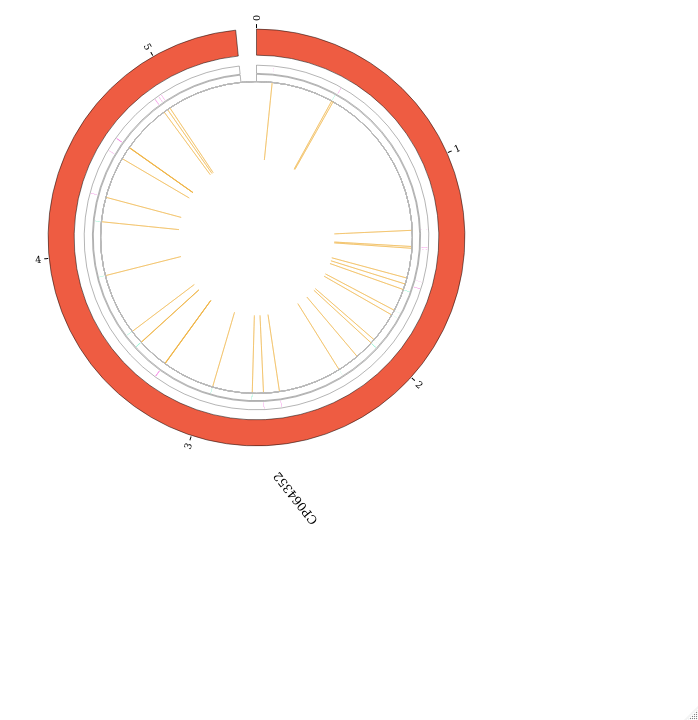
\includegraphics[width=0.8\linewidth]{figs/biocircos_ATCC43816.png}
	\label{fig:bioATCC43816}
\end{figure}

\begin{figure}[h]
	\centering
	\captionsetup{width=\linewidth}
	\caption[Gráfica biocircos para la cepa KpC11 de \textit{K. pneumoniae}]{Representación gráfica con BioCircos de los genes duplicados en el genoma de la cepa KpC11 de \textit{K. pneumoniae}.}
	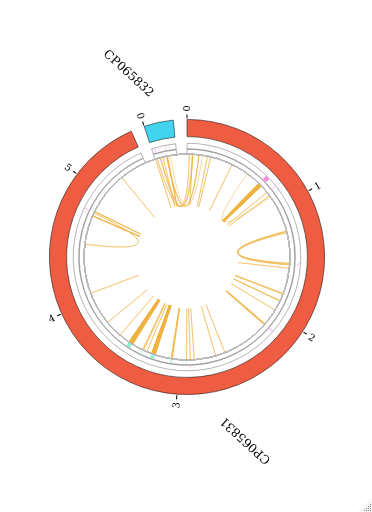
\includegraphics[width=0.8\linewidth]{figs/biocircos_KpC11.png}
	\label{fig:bioKpC11}
\end{figure}

\begin{figure}[h]
	\centering
	\captionsetup{width=\linewidth}
	\caption[Gráfica biocircos para la cepa KpPF25 de \textit{K. pneumoniae}]{Representación gráfica con BioCircos de los genes duplicados en el genoma de la cepa KpPF25 de \textit{K. pneumoniae}.}
	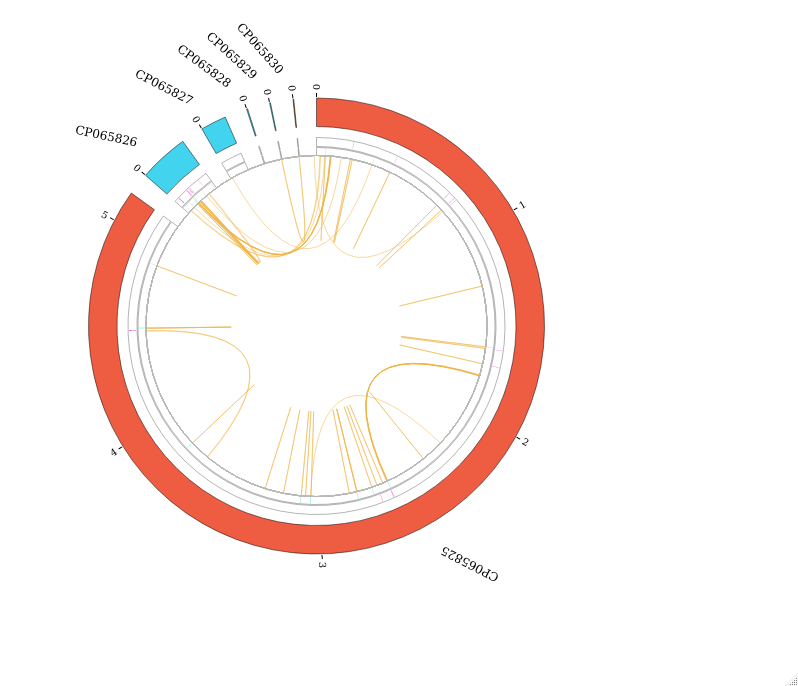
\includegraphics[width=0.8\linewidth]{figs/biocircos_KpPF25.png}
	\label{fig:bioKpPF25}
\end{figure}





\end{document}